%%%%%%%%%%%%%%%%%%%%%%%%%%%%%%%%%%%%%%%%%%%%%%%%%%%%%%%%%%%%%%%%%%%%%%%%%%%%%%%%
%2345678901234567890123456789012345678901234567890123456789012345678901234567890
%        1         2         3         4         5         6         7         8

\documentclass[journal]{IEEEtran}  % Comment this line out if you need a4paper

%\documentclass[a4paper, 10pt, conference]{ieeeconf}      % Use this line for a4 paper

% \IEEEoverridecommandlockouts                              % This command is only needed if 
                                                          % you want to use the \thanks command
\newcommand{\red}[1]{{\color{red} #1}}
% \overrideIEEEmargins                                      % Needed to meet printer requirements.

%In case you encounter the following error:
%Error 1010 The PDF file may be corrupt (unable to open PDF file) OR
%Error 1000 An error occurred while parsing a contents stream. Unable to analyze the PDF file.
%This is a known problem with pdfLaTeX conversion filter. The file cannot be opened with acrobat reader
%Please use one of the alternatives below to circumvent this error by uncommenting one or the other
%\pdfobjcompresslevel=0
%\pdfminorversion=4

% See the \addtolength command later in the file to balance the column lengths
% on the last page of the document

% The following packages can be found on http:\\www.ctan.org
\usepackage{graphics} % for pdf, bitmapped graphics files
\usepackage{graphicx}
\usepackage{epsfig} % for postscript graphics files
\usepackage{caption}
\usepackage{soul}
\usepackage[makeroom]{cancel}% for strikethrough
%\usepackage{mathptmx} % assumes new font selection scheme installed
\usepackage{subcaption}% subfigures 
% \usepackage[font=small]{caption}
\usepackage{times} % assumes new font selection scheme installed
\usepackage{amsmath} % assumes amsmath package installed
\usepackage{amssymb}  % assumes amsmath package installed
\usepackage{bbm}
\usepackage[nocomma]{optidef}
\usepackage{tabularx}
\usepackage{multirow}
\usepackage{tablefootnote}
\usepackage{bm}
\providecommand{\bm}{\pmb}

\usepackage{cite}
%\usepackage[caption=false]{subfig}
\usepackage{subcaption}
\usepackage{hyperref}
\usepackage{cleveref}
\usepackage{booktabs}
\usepackage{ntheorem}
\usepackage{sidecap}
\sidecaptionvpos{figure}{c}
\usepackage[font=small]{caption}
\captionsetup[figure]{name=Fig.} 
%\theoremstyle{break}
\theoremstyle{plain}
\theorembodyfont{\upshape}
\newtheorem{example}{Example}
\newtheorem{theorem}{Theorem}
\newtheorem{proof}{Proof}[theorem]
\newtheorem{corollary}{Corollary}[theorem]
% \numberwithin{example}{section}
\usepackage[dvipsnames]{xcolor}

\usepackage[ruled,vlined]{algorithm2e}

\newcommand\xqed[1]{%
  \leavevmode\unskip\penalty9999 \hbox{}\nobreak\hfill
  \quad\hbox{#1}}
\newcommand\demo{\xqed{$\square$}}

\usepackage{xcolor}
\newcommand\todo[1]{\textbf{\textcolor{red}{TODO: #1}}}

\DeclareMathAlphabet{\mathcal}{OMS}{cmsy}{m}{n}
\setlength{\textfloatsep}{3pt plus 0pt minus 3pt}
\setlength{\floatsep}{3pt plus 0pt minus 1pt}
\setlength{\intextsep}{3pt plus 0pt minus 1pt}
\setlength{\abovecaptionskip}{3pt plus 0pt minus 3pt}

\usepackage{comment}
\usepackage{dsfont}


% ---------- New Symbols and Commands -------------------------
% ---------- Standard Commands -------------
%\newcommand{\red}[1]{\textcolor{red}{#1}}

% utilities
\newcommand{\add}[1]{\textcolor{blue}{#1}}
% comments
\newcommand{\MT}[1]{\red{(MT: #1)}}

% ---------- new commands ------------------
\newcommand{\vect}[1]{\bm{#1}}		% vectors
\newcommand{\matr}[1]{\bm{#1}}		% matrices
\newcommand{\nR}[1]{\mathbb{R}^{#1}}		% real number
\newcommand{\nT}[1]{\mathbb{T}^{#1}}		% real number
\newcommand{\nN}[1]{\mathbb{N}^{#1}}		% real number
\newcommand{\define}{:=}			% define symbol
\newcommand{\modulus}[1]{\left| #1 \right|}	% abs
\newcommand{\matrice}[1]{\begin{bmatrix} #1 \end{bmatrix}}	% matrix
\newcommand{\smallmatrice}[1]{\left[\begin{smallmatrix} #1 \end{smallmatrix}\right]}	% matrix
\newcommand{\cosp}[1]{\cos \left( #1 \right)}	% cos with brace
\newcommand{\sinp}[1]{\sin \left( #1 \right)}	% sin with brace
\newcommand{\determinant}[1]{\text{det}\left(#1\right)} 	% determinant
\newcommand{\sgn}[1]{\text{sgn}\left( #1 \right)}			% signum
\newcommand{\atanTwo}[1]{{\rm atan2}\left( #1\right)}		% atan2
\newcommand{\acotTwo}[1]{{\rm acot2}\left( #1\right)}		% acot2
\newcommand{\upperRomannumeral}[1]{\uppercase\expandafter{\romannumeral#1}}	% roman numbers
\newcommand{\lowerromannumeral}[1]{\romannumeral#1\relax}
\newcommand{\vSpace}{\;\,}

%-----------Functions------------------------
\newcommand{\minEig}[1]{\lambda_{\text{min}}[#1]}
\newcommand{\maxEig}[1]{\lambda_{\text{max}}[#1]}
\newcommand{\transpose}{\top}


% --------- References ----------------------
\newcommand{\fig}{Fig.~}	% figure ref
\newcommand{\eqn}{Eq.~}	% equation ref
\newcommand{\tab}{Tab.~}	% table ref
\newcommand{\cha}{Chap.~}	% chapter ref
\newcommand{\sect}{Sec.~}	% section ref
\newcommand{\algo}{Algo.~}

% --------- Variables -----------------------

% General
\renewcommand{\frame}{\mathcal{F}}		% frame
\newcommand{\origin}{O}						% origin
\newcommand{\vX}{\vect{x}}					% x-axis
\newcommand{\vY}{\vect{y}}					% y-axis
\newcommand{\vZ}{\vect{z}}					% z-axis
\newcommand{\pos}{\vect{p}}				% position vector
\newcommand{\dpos}{\vect{v}}				% velocity vector
\newcommand{\rotMat}{\matr{R}}				% rotation matrix
\newcommand{\rotMatVectAngle}[2]{\rotMat_{#1}(#2)}	% rotation matrix representing the rotation about a vector of a certain angle
\newcommand{\vZero}{\vect{0}}				% vect/matr of zeros
\newcommand{\eye}[1]{\matr{I}_{#1}}
\newcommand{\zeros}[1]{\matr{0}_{#1}}

% World frame
\newcommand{\frameW}{\frame_W}			% world frame
\newcommand{\originW}{\origin_W}		% origin world frame
\newcommand{\xW}{\vX_W}				% x-axis world frame
\newcommand{\yW}{\vY_W}				% y-axis world frame
\newcommand{\zW}{\vZ_W}				% z-axis world frame

% Robot
\newcommand{\configRobot}{\vect{q}} % Robot configuration
\newcommand{\dconfigRobot}{\dot{\vect{q}}} % Robot configuration
\newcommand{\ddconfigRobot}{\ddot{\vect{q}}} % Robot configuration
\newcommand{\robotDoF}{n_q} % Robot dof
\newcommand{\massMatrix}{M(\configRobot)}
\newcommand{\coriolis}{C(\configRobot, \dconfigRobot)}
\newcommand{\error}[1]{\tilde{#1}}
\newcommand{\desired}[1]{#1^*}
\newcommand{\configRobotError}{\error{\vect{q}}} % Robot configuration
\newcommand{\dconfigRobotError}{\dot{\error{\vect{q}}}} % Robot configuration
\newcommand{\ddconfigRobotError}{\ddot{\error{\vect{q}}}} % Robot configuration
\newcommand{\configRobotDesired}{\desired{\configRobot}} % Robot configuration
\newcommand{\dconfigRobotDesired}{\desired{\dconfigRobot}} % Robot configuration
\newcommand{\ddconfigRobotDesired}{\desired{\ddconfigRobot}} % Robot configuration


% Object
\newcommand{\configObject}{\vect{o}} % Robot configuration
\newcommand{\dconfigObject}{\dot{\vect{o}}} % Robot configuration
\newcommand{\contact}{\gamma}
\newcommand{\objectDoF}{n_o} % Robot dof

% system
\newcommand{\state}{\vect{x}} % state
\newcommand{\dstate}{\dot{\vect{x}}} % state
\newcommand{\command}{\vect{u}} % state
\newcommand{\pose}{\vect{p}} % state
\newcommand{\robotState}{\state_{rob}}
\newcommand{\objectState}{\state_{obj}}
\newcommand{\drobotState}{\dot{\state}_{rob}}
\newcommand{\dobjectState}{\dot{\state}_{obj}}
\newcommand{\robotCoriolis}{\vect{b}_{r}(\configRobot, \dconfigRobot)}
\newcommand{\objectCoriolis}{\vect{b}_{o}(\configObject, \dconfigObject)}
\newcommand{\upperLimits}{\configRobot_{\text{upper}}}
\newcommand{\lowerLimits}{\configRobot_{\text{lower}}}
\newcommand{\weightScalar}[1]{w_{#1}}
\newcommand{\weightMatrix}[1]{\matr{W}_{#1}}
\newcommand{\commandTorque}{\boldsymbol{\tau}_{cmd}}
\newcommand{\externalTorque}{\boldsymbol{\tau}_{ext}}


% control theory
\newcommand{\inputSequence}{U}
\newcommand{\stateSequence}{X}
\newcommand{\trajectory}{\vect{\tau}}
\newcommand{\noise}{\vect{\epsilon}}
\newcommand{\variance}{\matr{\Sigma}}
\newcommand{\successState}{\mathcal{O}}
\newcommand{\successStateTraj}{\successState_{\trajectory}}
\newcommand{\gradientInput}{\nabla_{\inputSequence}}
\newcommand{\expectation}[1]{\mathbb{E}_{#1}}
\newcommand{\utility}{\exp( -\lambda J)}

% Sampling control
\newcommand{\traj}{X_t, U_t}
\newcommand{\success}{\mathcal{O}}
\newcommand{\policyParams}{\boldsymbol{\theta}}
\newcommand{\policy}{\pi_{\policyParams}}
\newcommand{\expPolicy}[1]{\mathbb{E}_{\policy} \left [#1\right]}
\newcommand{\succCondProb}{p(\success | \traj)}
\newcommand{\succProb}{p(\success = 1)}
\newcommand{\meanVector}{\boldsymbol{\mu}}

% barrier function
\newcommand{\safeSet}{\mathcal{C}}
\newcommand{\boundary}[1]{\partial #1}
\newcommand{\interior}[1]{\text{Int}(#1)}
\newcommand{\zbf}{h(x)}





\begin{document}

\title{
\add{Robust Sampling-based Control of Mobile Manipulators for Interaction with Articulated Objects}
}


\author{Giuseppe Rizzi$^1$, Jen Jen Chung$^2$,~\IEEEmembership{Member,~IEEE}, Abel Gawel$^3$, Lionel Ott$^1$, Marco Tognon$^1$,~\IEEEmembership{Member,~IEEE}, and Roland Siegwart$^1$,~\IEEEmembership{Fellow,~IEEE}% <-this % stops a space
\thanks{This work was supported by the European Union H2020 program under project PILOTING No H2020-ICT-2019-2 871542 and project HERON under grant agreement No 955356.}
\thanks{$^1$ Autonomous Systems Lab, ETH Z\"urich, Z\"urich 8092, Switzerland. {\tt\small\{grizzi\}@ethz.ch}}%
\thanks{$^2$ School of ITEE, The University of Queensland, Australia.}%
\thanks{$^3$ Huawei Technologies, Z\"urich, Switzerland.}%
}

% The paper headers                                                                                  
\markboth{IEEE Transactions on Robotics,~Vol.~X, No.~X, May~2022}%                              
{Rizzi \MakeLowercase{\textit{et al.}}: \remove{A Framework for Interaction Control of Mobile Manipulators} \add{Robust Sampling-Based Control of Mobile Manipulators for Interaction with Articulated Objects}}

% \IEEEpubid{0000--0000/00\$00.00~\copyright~2021 IEEE}
% Remember, if you use this you must call \IEEEpubidadjcol in the second                             
% column for its text to clear the IEEEpubid mark.                                                   



\maketitle
% \thispagestyle{empty}
% \pagestyle{empty}


%%%%%%%%%%%%%%%%%%%%%%%%%%%%%%%%%%%%%%%%%%%%%%%%%%%%%%%%%%%%%%%%%%%%%%%%%%%%%%%%
\begin{abstract}

In this work we investigate and deploy sampling-based control techniques for the challenging task of mobile manipulation \add{of articulated objects.} By their nature, manipulation tasks necessitate environment interactions which require the handling of non-differentiable switching contact dynamics. These dynamics represent a strong limitation for traditional gradient-based optimization methods such as Model Predictive Control (MPC) and Differential Dynamic Programming (DDP) \add{which often rely on heuristics for trajectory generation.} \emph{Sampling-based} techniques alleviate these constraints but do not ensure \add{robots' stability and input/state constraints either.} On the other hand, real-world applications in human environments require safety and robustness to unexpected events. For this reason, we propose a novel framework for safe robotic manipulation of movable \add{articulated} objects. \add{The framework} combines sampling-based control together with \emph{Control Barrier Functions} and \emph{Passivity Theory} that, thanks to formal stability guarantees, enhance the safety and robustness of the method. 
\add{We also provide the practical insights that} enable robust deployment of stochastic control using a conventional CPU. We deploy the algorithm on a 10-DOF mobile manipulator robot. 
%\add{A video of the experiments can be found  \href{https://youtu.be/Q1AohXmsLs4}{here}}.
Finally, we open-source our generic and multi-threaded implementation.
\end{abstract}


%%%%%%%%%%%%%%%%%%%%%%%%%%%%%%%%%%%%%%%%%%%%%%%%%%%%%%%%%%%%%%%%%%%%%%%%%%%%%%%%
\begin{IEEEkeywords}
Motion Control of Manipulators, Mobile Manipulation, Optimization and Optimal Control, Manipulation of Articulated Objects.
\end{IEEEkeywords}

\section{Introduction} \label{sec:introduction}
% Vision

There is a growing interest in deploying autonomous systems in unstructured environments to perform complex manipulation tasks for different applications like assistive service in the healthcare domain~\cite{cooper2020ari}, agrifoods~\cite{duckett2018agricultural}, and industrial inspection and maintenance~\cite{lattanzi2017review}. Mobile manipulator robots present a compelling choice to tackle these problems since they combine an unconstrained workspace with highly dexterous interaction capabilities. However, to fully exploit these capabilities, systems require planning and control algorithms that can generate fast, accurate, and coordinated reactive whole-body motions that account for multiple potential contacts with the environment. 

\subsection{Related Works}

% Existing methods
While traditional ``plan-and-act'' frameworks break down such tasks into subproblems that are easier to solve (e.g. reach, grasp, pull)~\cite{Murali2020}, they do not offer fast replanning, which is crucial for mobile manipulation in dynamic and uncertain environments.

With the recent advancements in artificial intelligence, reinforcement learning (RL) is a promising method to solve a range of robotic control tasks, including manipulation~\cite{finn2016deep}, as they learn an end-to-end representation of the optimal policy. However, real-world applications of RL typically require training times that are not practical for physical hardware and suffer from the well-known \textit{sim-to-real} gap~\cite{chebotar2019closing}. 
On the other side of the spectrum, Model Predictive Control (MPC) has gained broad interest in the robotics community thanks to its ability to deal with input constraints and task objectives by solving a multivariate optimization problem or using the \textit{principle of optimality}. 
MPC has been successfully applied to aerial robots~\cite{brunner2020trajectory}, autonomous racing~\cite{liniger2015optimization}, legged locomotion~\cite{grandia2019frequency}, and whole-body control~\cite{minniti2019whole}. 
Nevertheless, MPC requires a model that is locally differentiable with respect to the input and the state~\cite{buchli2017optimal}. On the other hand, manipulation tasks involve changes in the contact state causing sharp discontinuities in both the cost and system dynamics, thus directly violating the differentiability requirements. 


\begin{figure}[t]
\centering
\includegraphics[trim={0 0 0 100},clip,width=0.9\columnwidth]{framework_manipulation/figures/hardware/system_figure.pdf}
\caption{\textit{RoyalPanda}, a 10-DOF mobile manipulator while performing a door opening task.} \label{fig:royal_panda}
\end{figure}

% Performance : sampling control
Recently, sampling-based methods have emerged and advanced in theory and applications~\cite{lee_aggressive_2020,abraham_model-based_2020,williams_information_nodate,williams_information_2017,rajamaki_augmenting_2017}. 
In contrast to traditional MPC, sampling methods stem from a probabilistic interpretation of the control problem. 
Rather than solving a complex optimization problem, they rely on sampling system trajectories, referred to as \textit{rollouts}, and ``weighting'' them according to the cumulative cost so that only favorable trajectories survive the iterative sampling process. The only requirement is that it is possible to forward simulate the system evolution. This has been exploited to control camera motions for target tracking in drone racing~\cite{lee_aggressive_2020}, robot arm motions for manipulation tasks~\cite{abraham_model-based_2020}, and for generating aggressive driving maneuvers such as drifting~\cite{williams_information_nodate, williams_information_2017}. 

% Gap 
Demonstrations on real systems involving different physical interactions (e.g. a robot arm opening a drawer~\cite{abraham_model-based_2020}) have typically only been shown by breaking down the multi-contact task into stages and enforcing constraints when switching between them. 
This can limit the control envelope of the system and sacrifices solution optimality. For example, it is common practice to fix the gripper orientation between successive reach and pull stages and perform manipulation under a rigid grasp. In the presence of uncertainty and tracking errors, this often leads to high contact forces and dangerous behaviors.

% Safety : Barrier functions
In order to avoid safety-critical configurations often additional cost terms are formulating. While penalizing unsafe paths, they do not prohibit them. As a consequence, constraints fulfillment merely relies on sampling ``safe" trajectories. 
Recently \emph{Control Barrier Functions} (CBFs) have been introduced as a means to constrain the system to a safe set. The safe set defines the locus where all safety requirements are met, e.g. no self-collision happens and joint limits are fulfilled. CBFs are expressed as affine inequality constraints in the control input that, when satisfied point-wise in the candidate safe set, imply forward invariance of the set and hence safety \cite{ames2016control}.  This control method has been successfully deployed in safety-critical applications such as Adaptive Cruise Control and Lane Keeping \cite{vahidi2003research}, segway stabilization \cite{gurriet2018towards} and human-robot collaboration \cite{benzi2021optimization}.

% Stability : passivity
Last but not least, sampling-based methods do not ensure stability which, especially during autonomous interaction, is as important as performance. In this regard, we are interested in a stable interaction with an \emph{a priori} poorly known environment. This lack of knowledge might come from sensing limitations or a model mismatches. \emph{Passivity theory} has drawn attention in recent years as a way to analyze the stability of a controlled system. Intuitively, a passive system cannot produce more energy than the one it is provided with. A rather new approach to ensure \emph{passivity} is to use an auxiliary virtual system called \emph{energy tank} as a storing element containing the maximum energy budget available to perform the task. Energy tanks have been successful deployed in many robotics applications such as for impedance controllers with time-varying stiffness \cite{schindlbeck2015unified}, force-impedance control \cite{shahriari2018valve}, and lately with CBFs for controlling a robotic arm \cite{benzi2021optimization}.

\subsection{Contributions}

We propose a practical and robust receding horizon algorithm that achieves real-time whole-body control of a mobile manipulator using only a laptop CPU. Our work is based on an iterative sampling of control trajectories. Safety and stability are ensured through a sequential optimization problem that finds the closest policy to the optimized one, which enforces constraints and passivity of the autonomous system.

Our main contribution is a new framework for mobile manipulation which combines tools from stochastic optimization, safety-critical control, and passivity theory.
% Results
To demonstrate the applicability and effectiveness of this approach, we perform several ablation studies in simulation on a dynamical manipulator and deploy the full algorithm on our \textit{RoyalPanda} platform (a 7-DOF Franka Emika Panda arm mounted on the holonomic Clearpath Ridgeback base, \fig\ref{fig:royal_panda}) for a target reaching and door opening task. An open source implementation of our solution is provided at \url{https://git.io/Jtda7}.

In summary, the contributions of the present work are as follows:
\begin{enumerate}
    \item A framework for safe interaction-aware receding horizon control of a mobile manipulator,
    \item practical insights and a power-aware cost formulation focused on mobile manipulation tasks,
    \item an experimental evaluation of the effectiveness of the approach and of the contribution of each algorithmic component and hardware experiments showing its applicability to the real platform,
    \item an open source implementation of the proposed method including a multi-threaded sampling-based controller and an efficient quadratic program for addressing kinematic and dynamic constraints.
    \end{enumerate}

\subsection{Overview}

The remainder of the paper is organized as follows. In 
\sect \ref{sec:formulation} the manipulation problem is first formulated. In \sect \ref{sec:theory} we review the main theoretical background introducing receding horizon sampling-based control, the concept of barrier functions and energy tanks. These tools are combined in a unified control method in \sect \ref{sec:control_method}. We then evaluate the overall method in \sect \ref{sec:experiments} and conclude with hardware experiments. 

\add{I should stress that we find ZBF and Pass as good fit as they are safety modules working at the same level (joint velocities) as the sampling, thus they meld very well together.}

\section{Modeling and Problem Formulation} \label{sec:formulation}

In this work we consider the challenging task of manipulating articulated objects\footnote{We define articulated objects as non-actuated objects composed of more than one rigid part connected by joints allowing rotations or translations.} with a mobile manipulator through \textit{non-prehensile manipulation}. We define $\configRobot \in \nR{\robotDoF}$ and $\dconfigRobot \in \nR{\robotDoF}$ as the vectors of the robot configuration and its time derivative, respectively, where $\robotDoF \in \nN{}_{>0}$ is the robot's DOF.
Similarly, we describe the object configuration and corresponding time derivative by $\configObject \in \nR{\objectDoF}$ and $\dconfigObject \in \nR{\objectDoF}$, respectively, where $\objectDoF \in \nN{}_{>0}$ is the object's DOF. The system input $\command  \in \nR{\robotDoF}$ are the desired robot joint velocities $\dconfigRobotDesired$. The state vector is defined by,
\begin{equation}
    \state = [\configRobot^\transpose \vSpace 
      \dconfigRobot^\transpose \vSpace 
      \configObject^\transpose \vSpace
      \dconfigObject^\transpose ]^\transpose  \in \nR{2(\robotDoF + \objectDoF)}.
\end{equation}
The time evolution of the state is described by the following equation of motion:
\begin{equation} \label{eq:eom}
    \dstate = f(\state, \command) =  
    \begin{bmatrix}
      \dconfigRobot \\
      \matr{M}_r^{-1}(\matr{J}_{r}^\transpose \vect{f}_{ext} - \robotCoriolis + \vect{\tau}_{cmd}(\command)) \\
      \dconfigObject \\
      \matr{M}_o^{-1}(-\matr{J}_{o}^\transpose \vect{f}_{ext} - \objectCoriolis)
    \end{bmatrix},
\end{equation}
where $\matr{M}_r \in \nR{\robotDoF \times \robotDoF}$ and $\matr{M}_o \in \nR{\objectDoF \times \objectDoF}$ represent the inertia matrices while $\matr{J}_r(\configRobot) \in \nR{\robotDoF \times 3}$ and $\matr{J}_o(\configObject) \in \nR{\objectDoF \times 3}$ are the Jacobians at the robot and object contact point\footnote{Without loss of generality we consider single contacts to simplify the notation. Nevertheless, extension to the multi-contact case is straightforward.}, respectively.
$\matr{J}_r$ and $\matr{J}_o$ map the interaction force $\vect{f}_{ext} \in \nR{3}$ at the contact point into the efforts at the object and robot joints. Coriolis and gravity terms are denoted as $\robotCoriolis$ and $\objectCoriolis$. 
The joint torques, denoted by $\vect{\tau}_{cmd}  \in \nR{\robotDoF}$, are computed by a low-level velocity controller as a function of the velocity references $\command$. We define with  $\mathcal{X} \subseteq \nR{2(\robotDoF + \objectDoF)}$ and $\mathcal{U} \subseteq \nR{\robotDoF}$ the spaces of admissible states and inputs, respectively. 

%The control objective is to minimize the distance from an initial to final desired configuration through a stochastic feedback policy $\policy(\vect{x}_t)$ where $\boldsymbol{\theta}$ are the policy parameters and $T$ is the length of the receding time horizon.
The control objective is to find the feedback policy $\policy(\vect{x}_t)$ that minimizes the distance from an initial configuration to a final desired configuration, where $\boldsymbol{\theta}$ are the policy parameters, $T$ is the length of the receding time horizon, and $\vect{x}_t)$ is the system state at time $t$.
The \textit{distance} to the desired configuration must be defined for the specific problem and can be computed in a space different to $\mathcal{X}$ via an opportune mapping $h : \mathcal{X} \rightarrow \mathcal{H}$: 
\begin{mini}|s| 
{\policy}{\lim_{t \rightarrow \infty} || h(\state^*) - h(\state(t)) ||}{}{\label{eq:objective}}
\addConstraint{\dstate_t=f(\state_t, \command_t) \quad \forall \ t}{}{}
\addConstraint{\state_t  \in \mathcal{X}         \quad \forall \ t}{}{}
\addConstraint{\command_t \in \mathcal{U}        \quad \forall \ t}{}{}.
\end{mini}

%As an example, the manipulation task that we analyse consists of moving an articulated object to a desired configuration. 
In particular, in this work we address the problem of moving an articulated object to a desired configuration.
In this case the distance function $h(\vect{x})$ in \eqref{eq:objective} can be defined as:
\begin{equation}
   || h(\state^*) - h(\state(t)) || = || \configObject^* - \configObject ||_2,
\end{equation}
with $\configObject^*$ as the desired final configuration of the object. 
The optimal control problem subjected to constraints in \eqref{eq:objective} requires solving a complex minimization in a high dimensional and non-linear space. 
To facilitate the solving of \eqref{eq:objective}, additional \textit{surrogate objectives} are defined to introduce some bias towards the optimal solution. These objectives will appear as additional \textit{cost terms} that penalize specific configurations. 
The separate terms will be presented and explained in Section~\ref{sec:control_method}.


\section{Preliminaries} \label{sec:theory}

As the proposed method uses a combination of theoretical tools that span different applications and previous works, we present a short summary that can help the reader to better understand the remainder of the paper and build some preliminary background.

\subsection{Sampling-based control}
In contrast to deterministic policy optimization, we look at the optimal control problem \eqref{eq:objective} from a Bayesian perspective. This approach has many similarities with policy gradient methods used in reinforcement learning \cite{williams1992simple}. The key difference is that the method is used \emph{online} to iteratively update a parametric policy. While there are several avenues to derive the update equations, for example \emph{Variational Inference} \cite{lambert_stein_2020} or \emph{Free Energy} \cite{williams_information_2017}, here we will refer to \emph{Stochastic Control} (SC) and follow a Bayesian approach similar to \cite{levine2018reinforcement}. 

The control problem is formulated introducing an additional binary random variable $\successState$ whose value is $1$ when a trajectory is optimal, and $\successState = 0$ when it is not. Each trajectory is assigned a likelihood which depends on its cumulative cost. The optimal control objective is to find the optimal input parameters $\policyParams$ which maximize the success probability $\succProb$. In order to improve convergence, we optimize its logarithm, as it has high gradients in the domain where the probability is low: 
\begin{equation} \label{eq:bayesian_objective}
    \policyParams^* = \underset{\policyParams}{\arg\max} \log \succProb
\end{equation}
The success likelihood can be further expanded to make explicit its dependence on the policy parameters:
\begin{align}
        \succProb
        &= \int_{\policy} p(\successState | X_t, U_t; \state_t) p(X_t, U_t; \state_t) \\
        &= \int_{\policy}p(\successState | X_t, U_t) p(X_t| U_t) p(U_t) \label{eq:deterministic_dynamics}\\
        &= \int_{\policy}p(\successState | X_t, U_t) \policy(U_t) \\
        &= \expectation{\policy} [p(\successState | X_t, U_t)].
        \label{eq:input_to_params}
\end{align}
The step in \eqref{eq:deterministic_dynamics} follows from the assumption of deterministic dynamics and we drop the explicit dependence on $\state_t$ as this is already contained in the state sequence $X_t$. Any monotonically decreasing function $g(\cdot): \nR{} \rightarrow \nR{}_{>0}$ can be used to map costs to a \textit{pseudo success likelihood}:
\begin{equation}
p(\successState = 1| X_t, U_t) \propto g(J(X_t, U_t)) \triangleq \mathcal{J}.
\end{equation}
Often the exponential function is used:
\begin{align*}
    \expectation{\policy} [p(\successState | X_t, U_t)]  
    &= \expectation{\policy} \left[ \mathcal{J}(X_t, U_t) \right] \\
    &= \expectation{\policy} \left[ \exp (-\lambda J(X_t, U_t)) \right],
\end{align*}
where the higher the $\lambda$, the lower the cost needs to be in order to be mapped to a small \textit{success likelihood}. To optimize the objective in \eqref{eq:bayesian_objective} we perform gradient descent:
\begin{equation}
    \policyParams^{i+1} 
    = \policyParams^i + \rho \nabla_{ \policyParams}\log \expectation{\policy} [\mathcal{J}(X_t, U_t)].
\end{equation}

We choose the exponential function to map costs to likelihoods and model the policy with a Gaussian distribution which is parametric in the mean $U_t \sim \{\mathcal{N}(\meanVector_t, \variance), \mathcal{N}(\meanVector_{t+1}, \variance), \dots, \mathcal{N}(\meanVector_{t+T-1}, \variance)\} = \policy$, with $\policyParams =  \{\meanVector_t, \meanVector_{t+1}, \dots, \meanVector_{t+T-1}\}$. $\variance \in \nR{n_u \times n_u}$ is the diagonal covariance matrix of the multinomial distribution. The derivation of the gradient step equation for this particular design choice can be found in Appendix~\ref{sec:app_derivation_policy_gradient}. In the end, we obtain the following update equation for the $k^{\text{th}}$ mean vector:
\begin{equation}
    \meanVector^{i+1}_{k} = \meanVector^{i}_{k} +  \rho \variance^{-1} \frac{\expPolicy{\utility \noise_k }}{\expPolicy{\utility}}  \label{eq:alpha_assumption},
\end{equation}
where $\noise_k = \command_k - \boldsymbol{\mu}_k$ is the random policy perturbation at time index $k$.
The step size can be decoupled from the noise variance $\rho = \alpha \variance $. Finally the expectation can be estimated empirically via Monte Carlo sampling, obtaining the final policy update rule:
\begin{align} \label{eq:update_rule}
  \meanVector^{i+1}_{k} &= \meanVector^{i}_{k} + \alpha  \sum \limits_{n=1}^{N}  \omega_l \noise_{k}^{l} \\
  \omega_l  &\approx \frac{\exp ( -\lambda J_l )}{\sum \limits_{l=1}^{N} \exp ( -\lambda J_l)}, \label{eq:weighting}
\end{align}
where $N$ is the number of sampled rollouts. 
The input sequence applied to the system is then chosen as the \emph{maximum-likelihood-estimator} of the policy, which is trivially given by its mean: $U^*_t = \policyParams$.

\subsection{Control Barrier Functions}
It is desirable to design a controller that mediates performance and safety. \emph{Control Barrier Functions} have been recently introduced as a means to unify these objectives. This theory is based on the concept of \emph{forward invariance} of a safe set $\safeSet $, which is where safety conditions are met. A set $\mathcal{S}$ is called \emph{forward invariant} if for every $\vect{x}_0 \in \mathcal{S},\ \vect{x}(t) \in \mathcal{S}$ for every $t$. A differentiable function $\zbf$  characterizes the safe set, such that:
\begin{align*}
    \safeSet &= \{ \vect{x} \in \nR{n} : \zbf \geq 0 \}, \\
    \boundary{\safeSet} &= \{ \vect{x} \in \nR{n} : \zbf = 0 \}, \\
    \interior{\safeSet} &= \{ \vect{x} \in \nR{n} : \zbf > 0 \},
\end{align*}
where $\boundary{\safeSet}$ and $\interior{\safeSet}$ denote the boundary and interior of the safe set, respectively.
The function $\zbf$ is a \emph{Zeroing Barrier Function} (ZBF) for the set $ \safeSet $ if there exist a $\gamma > 0$ and a set $\mathcal{D}$ with $\safeSet \subseteq \mathcal{D} \subset \nR{n}$ such that, $\forall \  \vect{x} \  \in \mathcal{D}$, 
\begin{equation} \label{eq:zbf_constraint}
    \dot{h}(\vect{x}) \geq -\gamma \zbf.
\end{equation}
The existence of a ZBF implies the forward invariance of $\safeSet$ \cite{ames2016control}. Furthermore, defining the ZBF on a larger set than $\safeSet$ allows the system to be more robust to model perturbations\footnote{As shown in \cite{ames2016control}, CBFs induce an asymptotically stable behavior towards the safe set $\safeSet$. This property is particularly useful when disturbances bring the system outside the constraints.}. The condition in \eqref{eq:zbf_constraint} can be rewritten for a controlled affine system as,
\begin{equation}
    \sup_{\vect{u} \in \mathcal{U}} \left[ \frac{\partial h }{\partial \vect{x}} (f(\vect{x}) + g(\vect{x})\vect{u}) + \gamma \zbf \right] \geq 0, \forall \vect{x} \in \mathcal{D}.
\end{equation}
When this inequality is fulfilled by the control input, the system will be made forward invariant. 
As the constraint is affine in the control input, it can be solved via a quadratic optimization problem (QP). The advantage of a QP is that it allows trading-off performance and safety through ZBF. When a feed-forward control is available from a nominal controller a minimum perturbation on the feedforward command vector $\vect{u}_{ff}$ can be found through the following QP \cite{ames2019control}:
\begin{argmini}|s| 
{\vect{u} \in \nR{n}}{\frac{1}{2} ||\vect{u} - \vect{u}_{ff}||}{}{\label{eq:cbf-const}}
\addConstraint{\dot{h}(\vect{x}) \geq \gamma \zbf}{}{}.
\end{argmini}


However, in practice the control input is constrained to the feasible set and therefore controlled invariance cannot generally be guaranteed for the real system. As a remedy, we add input limits as hard constraints while softening CBF constraints with the use of slack variables\footnote{In comparison, \cite{gurriet2018towards} addresses this issue by finding \emph{viable sets}. A set is said to be \emph{viable} if there exists a feasible input which makes the set forward invariant at all times. Efficient computation of viable sets is still an open research area and is mostly applied to simpler systems due to the high computational requirements.}.

\subsection{Passivity and Energy Tank}
It is important that the autonomous system preserves passive behavior during interaction. Consider a system with state $\state \in \nR{n}$, input $\vect{u} \in \nR{m}$ and output $\vect{y} \in \nR{m}$. 
This system is said to be \emph{passive} w.r.t $(\vect{u},\vect{y})$ if for all inputs and initial states, there exists a positive semidefinite \emph{storage function} $S: \nR{m} \rightarrow \nR{}_+$ such that for any time $\sigma$,
\begin{equation}
    S(\vect{x}(\sigma)) - S(\vect{x}(0))\leq \int\limits_{0}^{\sigma} \vect{u}^T \vect{y}\ dt.  
\end{equation}
In other words, no additional energy can be produced other than what is flowing to the system through the \textit{power port} $(\vect{u},\vect{y})$.
For an autonomously controlled system (including the environment it is interacting with), this condition translates to, 
\begin{equation}
    \dot{S} \leq P_{in} \leq 0,
\end{equation}
where $P_{in}$ is the power flowing into the system. As shown in \cite{shahriari2018valve}, autonomous passivity can be enforced by interconnecting the controlled system with a secondary passive system, called the \emph{energy tank}, whose energy is bounded. The energy tank has state $x_t \in \nR{}$ and storage function $S(t) = \frac{1}{2} x_t^2 \in \nR{}$, with $S_t(0)$ as its initial value. Its time evolution is described by,
\begin{equation}
\begin{cases}
\dot{x}_t &= u_t(t) \\
y_t(t) &= \frac{\partial S}{\partial x_t} = x_t(t),
\end{cases}
\end{equation}
where $(u_t(t), y_t(t))$ is the power port through which the tank can exchange energy with the interconnected system. By interconnecting the controlled system with the tank, a passivity-violating control action will result in the depletion of the tank. When the tank has no energy left, passive behaviors cannot be implemented anymore. The interconnection can be implemented as follows:
\begin{equation}
\begin{cases}
    u_t(t) &= \vect{A}^T(t) \vect{u} \\
    \vect{y} &= \vect{A}(t) y_t(t),
\end{cases}
\end{equation}
where $\vect{A}(t) \in \nR{m}$ is defined as,
\begin{equation} \label{eq:tank_modulation}
    A(t) = \frac{\boldsymbol{\gamma}(t)}{x_t(t)}.
\end{equation}
The modulation variable $\boldsymbol{\gamma}(t) \in \nR{m}$ can be chosen to implement the desired value of $\vect{y}$. With the above equations one can easily show that $\dot{S} = u_t^T y_t = \vect{u}^T \vect{y}$ and therefore that power is either injected into or extracted from the tank. As visible in \eqref{eq:tank_modulation} there is a singularity when the tank is empty and the desired behavior can no longer be implemented. 
Therefore it is necessary to ensure that $S(x(t)) \geq \epsilon > 0, \ \forall t$.

\section{Control Method} \label{sec:control_method}

In this section we combine sampling, barrier functions and energy tank into a novel model-based control framework for robust and safe interaction control. We use the presented sampling method to generate joint velocity command sequences that optimize a task-dependent objective in a receding horizon fashion. We encode a set of tasks and safety-related objectives as different cost terms. Nevertheless, sampling does not inherently provide guarantees and therefore we need a method to enhance safety. We address this problem using an optimization problem as a non-invasive way to change the command sequence when constraints are not fulfilled. In particular, we solve a \textit{sequential} optimization problem (QP), which takes as input a command sequence and the starting state, and returns a modified command-state sequence satisfying all constraints. Nevertheless, as the expensive rollout sampling procedure often limits the rate of the controller, a portion of this input sequence must be executed in \textit{open-loop} which can be unsafe in dynamic environments and for low sampling rates. On the other hand, the QP can be efficiently solved at almost the same rate as the low-level controller. To this end, we propose a \emph{cascaded control} architecture composed of an inner loop where the policy is updated at a low-rate and an outer loop  where the low-level controller tracks the policy commands. In the outer loop a QP is solved for the current state-input pair in order to find the best input according to the latest received measurements. In the inner loop the same QP is solved for each state-input pair of the optimal rollout trajectory.
In other words, the optimization problem is solved:
\begin{itemize}
    \item \textit{sequentially}, for each command in the optimal input-state trajectory to ``sanitize" the sampling-based controller output wherever constraints might be violated,
    \item \textit{point-wise}, for each command executed by the low-level controller, in order to account for different control rates.
\end{itemize}
The complete high-level schematic of the full framework is depicted in \fig~\ref{fig:block_scheme}. Sequential and point-wise optimizations are denoted as Sequential FILTER-QP and FILTER-QP respectively and belong to the \textit{Trajectory Filtering} block of \fig~\ref{fig:block_scheme}. 

The full method is amenable to different variants. In particular, by turning on/off filtering in the outer or inner control loop, we can synthesize four possible controller implementations. In the following we define with $\Pi_{*}$ each controller where $*$ can be $N,\ O,\ I,\ IO$:
\begin{itemize}
    \item[$\Pi_{N}$:] relies exclusively on a stochastic controller to generate velocity commands, namely the \textit{Trajectory Filtering} block is completely missing and the sampled input trajectory is tracked as it is by the low-level velocity controller,
    \item[$\Pi_{O}$:] a FILTER-QP is used to filter the instantaneous input command to be tracked by the low-level velocity controller,
    \item[$\Pi_{I}$:] the Sequential FILTER-QP is used to filter the full optimized command trajectory in a sequential manner but no FILTER-QP is used in the outer control loop,
    \item[$\Pi_{IO}$:] the full cascaded architecture is deployed, combining the previous two methods.
\end{itemize}

\begin{figure}[t!]
\centering
\vspace{-0.5cm}
% \hspace*{-1.5cm}
\includegraphics[trim=120 0 50 0, clip, width=0.95\columnwidth] {figures/schemes/receding_horizon_paper.pdf}
\caption{The figure shows an high-level schematic of the method. The \textcolor{blue}{\textbf{blue}} variables represent the information available at the new optimization step. Some information is reused from the previous iteration to warm start the sampling procedure as shown in \textcolor{darkgreen}{\textbf{dark green}}. The cascaded control scheme is composed by a low-rate input sequence generation and an high-rate velocity command tracking blocks. We propose to modify the input sequence in both blocks through the Sequential FILTER-QP and FILTER-QP as a way to add guarantees to the command sequences generated via sampling and stochastic optimization.} \label{fig:block_scheme}
\end{figure}


In the following we present our cost formulation for the manipulation task. This is used in the sampling procedure to weight different trajectory samples and drive the robot to a successful task execution. Then, we encode safety requirements in the form of ZBFs. These allow us to formulate an optimization problem that ensures forward invariance with respect to the safe set when joint velocities are accurately tracked.

While the safety objectives here are formulated on a kinematic level (obstacle avoidance, joint and cartesian limits), we are also interested in the robustness of the dynamical system during interaction, especially in cases of unexpected events that could compromise its stability. For this purpose, we complete the proposed framework with a passivity analysis and use an energy tank to bound the energy dissipated during the manipulation task. Passivity is guaranteed in the form of an additional constraint in the quadratic program and therefore naturally fits the proposed framework.

\subsection{Sampling-based Control}
The sampling-based framework offers the freedom to directly plan in torque space or use position/velocity control and defer tracking to a low-level controller. In fact, directly planning in the joint space allows us to account for objectives which are not in the operational control space such as joint limits and self-collision avoidance. The internal model used to sample trajectory rollouts has the same form as in \eqref{eq:eom}. Joint velocity commands are sampled and then translated to motor torques:
\begin{equation}
    \vect{\tau}_{cmd} = \matr{K}_{D} (\command - \dconfigRobot) + \robotCoriolis,
\end{equation}
with an appropriate choice of the positive-definite diagonal gain matrix $\matr{K}_{D} \in \nR{\robotDoF\times\robotDoF}$. 

\subsection{Cost Shaping}
As described in Section~\ref{sec:formulation}, the control objective is to drive the system to minimize a task-dependent cost function over time. Furthermore, as state constraints are not explicitly taken into account by the formulation, a common heuristic is to penalize deviations from feasible states in the cost function. In the following we define several cost components associated with the different high-level objectives and constraints.
We denote by $\mathds{1}[\cdot]$ the \textit{indicator function} such that,
\begin{equation}
    \mathds{1}[x] = 
    \begin{cases}
    1 & \text{if } x \text{ is True} \\
    0 & \text{otherwise}.
    \end{cases}
\end{equation}
In the following we drop from the notation the dependence on the current state. We use $\weightMatrix{}$ to denote positive semidefinite weight matrices and $\weightScalar{}$ for non-negative scalar parameters. Note that input constraints are not treated here as additional cost terms as the non-linear dynamics can be augmented with a function that projects the sampled inputs into the feasible set $\mathcal{U}$.

\paragraph{Target reaching} in the target reaching task, the goal is to bring a frame attached to the robot (generally the end-effector frame) to a desired pose. We define with $\matr{T} \in SE(3)$ and $\matr{T}^* \in SE(3)$ the current and desired target frame pose, respectively. The \textit{tracking cost} is computed as a weighted distance in the tangent space to $SE(3)$ using the logarithmic mapping~\cite{blanco2010tutorial}:
\begin{equation} \label{eq:tracking_cost}
     c_{t} = || \log(\matr{T} - \matr{T}^{*}) ||^2_{\weightMatrix{t}}.
 \end{equation}
 
 \paragraph{Collision avoidance} let $\contact \in \{0, 1\}$ represent an auxiliary variable which is equal to 1 when the manipulator is in contact with the environment. The value of $\contact$ can be computed searching for collisions between bodies. 
 $\contact$ is used to avoid collisions during contact-free motions of the end-effector. 
 The \textit{contact cost} is defined as,
 \begin{equation}
     c_{\contact}= \weightScalar{\contact} \contact(\state).
 \end{equation}

 \paragraph{Joint position limits} the manipulator is subject to physical joint limits. These can be addressed by introducing a cost component that penalizes violation of the constraints. We define the \textit{joint limits cost} with:
 \begin{align}
     &c_{j} = \mathds{1}[\configRobot > \upperLimits](\weightScalar{j} + ||\upperLimits - \configRobot||^2_{\weightMatrix{js}}) + \nonumber\\ 
     &\qquad\mathds{1}[\configRobot < \lowerLimits](\weightScalar{j} +  || \configRobot - \lowerLimits||^2_{\weightMatrix{js}}), 
 \end{align}
 where the scalar $\weightScalar{j}$ is a constant cost added when the limit is violated. The matrix $\weightMatrix{js}$ adds a quadratic term in the limit violation. This was shown in~\cite{williams_information-theoretic_2018} to help the controller find its way back if poor sampling brings the system outside of the joint position limits.
 
 \paragraph{Arm reach} we introduce an additional term that penalizes configurations where the arm's end-effector moves excessively relative to the base 2D placement. This helps to bias solutions where base motion is preferred over stretching the arm which can lead to singular configurations. The translation vector from the end-effector frame $\mathcal{E}$ to the arm base frame $\mathcal{B}$ is defined with the vector $\vect{p}_{\mathcal{B}\mathcal{E}} \in \nR{3}$. The current reach is then $r_{\text{curr}} =  \vect{p}_{\mathcal{B}\mathcal{E}}^T \matr{P} \vect{p}_{\mathcal{B}\mathcal{E}}$. The projection matrix $\matr{P} = \text{diag}(1, 1, 0) \in \nR{3 \times 3}$ makes sure that the reach is only computed in the 2D plane. Given a maximum reach $r_{\text{max}} \in \nR{}_{\geq 0}$, the \textit{reach cost} is then defined by:
 \begin{equation}
   c_r = \mathds{1}[r_{\text{curr}} > r_{\text{max}}] (\weightScalar{r} + \weightScalar{rs}(r_{\text{curr}} - r_{\text{max}})^2).    
 \end{equation}

 \paragraph{Self-collision avoidance} similarly to arm reach, self-collision avoidance can be implemented as an additional cost term which is active when the distance between a pair of frames is less than a pair-dependent threshold. Given the distance between two frames $d_{ij}$ and a threshold $d^{min}_{ij}$ the self-collision cost for the pair is:
 \begin{equation}
   c_{sc} = \sum_{ij, i \neq j} \mathds{1}[d_{ij} < d^{min}_{ij}] (\weightScalar{r} + \weightScalar{rs}(d^{min}_{ij} - d_{ij})^2).    
 \end{equation}
 
 \paragraph{Object manipulation} in the manipulation task the goal is to change the state of an articulated object through interaction. The \textit{manipulation cost} penalizes deviations from the target object configuration $\configObject^{*}$,
\begin{equation}
    c_o(\configObject; \weightMatrix{o}) = || \configObject - \configObject^{*}||^2_{\weightMatrix{o}}.
\end{equation}
\paragraph{Power minimization} we propose a new cost component that takes into account the power dissipated to perform the task. In fact a successful interaction (i.e., opening the door) could happen in multiple ways, however trajectories that dissipate low power are most efficient as they do not act against the environment and robot kinematic constraints. We leverage the fact that as rollouts are performed in simulation, the joint torque generated through interaction can be easily computed by summing the contribution of each force $\vect{f}_c \in \nR{3}$ at each contact point $c$:
\begin{equation}
\boldsymbol{\tau}_{ext} = \sum\limits_{c} \matr{J}_c^T \vect{f}_c,    
\end{equation}
where $\matr{J}_c$ is the contact Jacobian. The power dissipated during the task is therefore $-\boldsymbol{\tau}_{ext}^T\command$, which is positive when acting ``against" the environment. The cost associated with power penalization is:
\begin{equation}
   c_p = \weightScalar{p} \cdot \max(0, - \boldsymbol{\tau}_{ext}^T\command - p_{max}),      
 \end{equation}
where $p_{max}$ is the maximum power that can be dissipated during the task.

\subsection{Cost Scheduling}
The manipulation task consists of two phases. In a first phase the manipulator reaches an estimated contact point, allowing for a fast and successful exploration in the following interaction phase. In the second phase, the goal is to bring the object to the desired state while keeping the end-effector close to the contact location. This switch is manually enabled by turning on the object manipulation cost $c_o$ after a successful approach. Reducing the end-effector position penalty during the manipulation phase allows the controller to choose a trajectory that fully exploits the contact dynamics by changing the hand pose.

%This approach is in contrast with previous works where manipulation generally follows a prescribed grasping state~\cite{abraham_model-based_2020}. Grasping introduces a kinematic constraint that, while reducing the optimal control search space, does not allow for more flexible, contact-based behaviors to emerge such as pulling, pushing or sliding. 

\subsection{Barrier Functions}
In the previous subsection a combination of cost components were introduced in order to address both performance and safety. The variety of objectives makes the cost landscape highly complex such that trading off performance against safety objectives can be quite challenging and tedious. Furthermore, as already stressed, sampling does not provide any formal guarantee that constraints encoded in the form of additional cost terms will be satisfied. Therefore, we look at how barrier functions can encode safety-critical constraints. As described in \cite{benzi2021optimization}, a simple ZBF can be derived for each joint to keep it between its lower and upper bounds, $q_i^-$ and $q_i^+$, respectively:
\begin{equation}
h_{ql}^i = \frac{(q_i^+ - q)(q - q_i^-)}{(q_i^+ - q_i^-)}\;.
\end{equation}

In the following we treat the safety requirements associated to robot frames and denote with $\vect{p}_{\mathcal{A}} \in \nR{3}$ the position of a generic robot frame $\mathcal{A}$ computed through forward kinematics. The ZBF constraint can then be derived using the differential kinematics equation,
\begin{equation}
    \dot{\vect{p}}_{\mathcal{A}} = \matr{J}^{lin}_{\mathcal{A}} \dconfigRobot\;,
\end{equation}
with $\matr{J}^{lin}_{\mathcal{A}}$ being the linear Jacobian associated with frame $\mathcal{A}$ and assuming that joint velocities are accurately tracked. 

The self-collision safe set can be obtained by approximating potentially colliding frames with non-intersecting spheres. Then the self-collision ZBF is defined as,
\begin{equation}
    h_{sc}^{ij} = \frac{1}{2}(||\vect{p}_{\mathcal{C}_i} - \vect{p}_{\mathcal{C}_j}||^2 - d_c^2),
\end{equation}
where $d_c = r_i + r_j$ is the sum of the radius of the two collision spheres associated with the $i$\textsuperscript{th}  and $j$\textsuperscript{th} collision pair frames. Note that we can similarly encode arm reach limits. In fact, the following is a valid ZBF, positive only when the end-effector is within the prescribed maximum reach $r_{max}$ with respect to the arm base,
\begin{equation}
    h_{ar} = \frac{1}{2}(r_{max}^2 - (\vect{p}_{\mathcal{E}} - \vect{p}_{\mathcal{B}})^T \vect{P} (\vect{p}_{\mathcal{E}} - \vect{p}_{\mathcal{B}}) ).
\end{equation}
The projection matrix $\vect{P} = \text{diag}(1, 1, 0) \in \nR{3 \times 3}$ makes sure that the reach is only computed in the 2D plane. This prevents the arm from stretching out and reaching singular configurations. Each of these ZBFs translates to a constraint of the form in \eqref{eq:cbf-const} which is affine in the commands. 

As described in \sect \ref{sec:theory}, we can formulate a quadratic program to find the command which is the closest to the sampled one while also satisfying the ZBF constraints previously introduced:
\begin{mini}|s| 
{\tilde{\vect{u}}_t, \boldsymbol{\delta}}{||\tilde{\vect{u}}_t - \command_t||^2 + \boldsymbol{\delta}^T \matr{\Gamma} \boldsymbol{\delta}\quad \text{(FILTER-QP)}}{}{\label{eq:cbf-qp}}
\addConstraint{\dot{h}^i_{ql} \geq -{h}_{ql} + \delta^i_{ql} \quad \forall \ i \in [1,  m] }{}{\ \text{(Joint Limits)}}
\addConstraint{\dot{h}^{ij}_{sc} \geq -{h}_{ij} + \delta^{ij}_{sc} \quad \forall \ (i,j) \in \mathcal{I}}{}{\ \text{(Self Collision)}}
\addConstraint{\dot{h}^i_{ar} \geq -{h}_{ar} + \delta^i_{ar}}{}{\ \text{(Arm Reach)}}
\addConstraint{\tilde{\vect{u}}_t \in \mathcal{U}}{}{ \text{\ (Input Limits)}},
\end{mini}
where $\boldsymbol{\delta}$ is the vector of slack variables and $\matr{\Gamma}$ is a positive definite diagonal matrix weighting the slack variable penalization whose dimensions depend on the number of implemented soft constraints. Finally, the set denoted by $\mathcal{I}$ is the set of collision link pairs.  We name this problem FILTER-QP as it changes the control input only if it is unsafe. Instead of simply applying this optimization point-wise, we can \emph{filter} the full input sequence in a sequential manner. After a policy update and for each time step, a FILTER-QP is solved. The newly computed command is applied to advance to the next step in the horizon and obtain the next system state from which the constraint equation can be updated. We call this procedure Sequential FILTER-QP and describe it in \algo \ref{algo:sequential_qp}. The resulting filtered optimal input sequence $\bar{U}^*_t$ is then also used to warm-start the nominal policy for the next round of rollout sampling (see \fig \ref{fig:receding_horizon}). The reader can also refer to \fig~\ref{fig:block_scheme} for a schematic representation of the complete feedback control loop.

\begin{algorithm}
\caption{Sequential FILTER-QP \label{algo:sequential_qp}}
\KwData{optimal input sequence $U^*_t = \{ \command^*_t, \dots, \command^*_{t+T-\Delta t}\} = \{\boldsymbol{\mu}_t, \dots, \boldsymbol{\mu}_{t+T-\Delta t}\}$ , current state $\vect{x}_t$, simulation steps $K$
%tank state $x_t$
}
\KwResult{filtered input trajectory $\bar{U}^*_t$}
$\vect{x} \gets \vect{x}_t$\;
$\command \gets \command^*_t$\;
$k \gets 0$\;
\While{$k < K$}{
  $\bar{\command}_{t+k\Delta t} \gets \text{FILTER-QP}(\vect{x}, \command, \boldsymbol{\tau}_{ext})$ \hfill (\eqn \ref{eq:cbf-qp}) \\
  $\vect{x}, \boldsymbol{\tau}_{ext} \gets $Step Simulation \hfill (\eqn \ref{eq:eom})\\
  %$x_t \gets$ Integrate Tank \hfill (\eqn \ref{eq:tank_dynamics}) \\
  $k = k + 1$ \\
  $\command \gets {\command}^*_{t + k\Delta t}$
}
\end{algorithm}

\subsection{Energy Tank}
While the optimization in \eqref{eq:cbf-qp} enhances the safety of the system we still lack stability guarantees. As described in \sect \ref{sec:theory}, energy tanks can be used to make the system \emph{passive} and thus ensure stability. Inspired by the work in \cite{benzi2021optimization} and \cite{shahriari2018valve}, this adaptation naturally fits the control method we have developed so far. Let us consider the dynamic manipulator as described in \eqref{eq:eom}. Furthermore, the system uses a dynamically compensated PI velocity controller: 
\begin{equation} \label{eq:low-level-control}
\commandTorque = \coriolis \dconfigRobotDesired + g(\configRobot) - \matr{K}_D \dconfigRobotError - \matr{K}_I \int_{0}^{\sigma} \dconfigRobotError\ dt,
\end{equation}
with the auxiliary error variable $\configRobotError =  \configRobot - \configRobotDesired$. If we augment the the optimization problem in \eqref{eq:cbf-qp} with the energy constraint:
\begin{equation}\label{eq:pass_const}
    \int\limits_{0}^{\sigma} \boldsymbol{\tau}_{ext}^T \dconfigRobotDesired \ dt \geq -S(0),
\end{equation}
where $S(0)$ is the initial energy stored in the tank, then the following stability result holds:

\begin{theorem}[Controlled System Stability]
If the optimization problem FILTER-QP satisfies constraint \eqref{eq:pass_const}, then the controllers $\Pi_O$ and $\Pi_{IO}$ make the system \eqref{eq:eom} passive and therefore stable. 
\end{theorem}


\begin{proof}
We start by augmenting the system model with a virtual tank. We now need to define through which \emph{power ports} the tank exchanges energy with the rest of the system. To this end, we perform a passivity analysis of the \emph{real} system. We first define the robot energy as, 
\begin{equation}
    S_{robot} = \frac{1}{2} \dconfigRobotError^T \massMatrix \dconfigRobotError + \frac{1}{2} \configRobotError^T \matr{K}_P \configRobotError.
\end{equation}
In order to study the passivity of the system, we need to derive the robot energy dynamics $\dot{S}_{robot}$. A complete derivation can be found in the Appendix~\ref{app:passivity_analysis}. It turns out that:
\begin{equation}
    \dot{S}_{robot} = \dconfigRobotError^T \externalTorque - \dconfigRobotError^T \matr{K}_D \dconfigRobotError \leq \dconfigRobotError^T \externalTorque. 
\end{equation}
The power flow through the external torque has indefinite sign and can lead to a loss of passivity. Since the environment is passive, there exists an environment energy $\dot{S}_{env}$ such that~\cite{shahriari2018valve},
\begin{equation}
    \dot{S}_{env} \leq -\dconfigRobot^T \externalTorque.
\end{equation}
The energy tank is finally connected to the system through the power port $(\dconfigRobot^*, \externalTorque)$ and therefore,
\begin{equation} \label{eq:tank_dynamics}
\dot{S}_{tank} = \dconfigRobot^{*T} \externalTorque. 
\end{equation}
Then, the energy evolution of the autonomous system, composed of robot, tank and environment is,
\begin{equation}
\begin{aligned}
    \dot{S}_{tot} &= \dot{S}_{robot} + \dot{S}_{tank} + \dot{S}_{env} \\
    &\leq \dconfigRobotError^T \externalTorque + \dconfigRobot^{*T} \externalTorque - \dconfigRobot^T \externalTorque \leq 0,
\end{aligned}
\end{equation}
showing the system's passivity.
Intuitively, the increase of the robot's energy is compensated with a reduction of the tank's energy. As the tank energy is limited and bounded from below, passivity is ensured if,
\begin{equation}
    S(t) = S(0) + \int_{0}^{\sigma} \boldsymbol{\tau}_{ext}^T \dconfigRobotDesired \ dt  \geq 0
\end{equation}
recovering the constraint in \eqref{eq:pass_const} and therefore concluding the proof.
\end{proof}
In practice, the constraint in \eqref{eq:pass_const} is formulated as
\begin{equation}
    \int_{0}^{\sigma} \boldsymbol{\tau}_{ext}^T \command \ dt \geq \epsilon - S(0),
\end{equation}
where $\epsilon$ is a positive minimum residual energy to avoid the singularity that the tank suffers when it is completely depleted.  



\section{Practical Aspects}

We address here some issues that arise when implementing the described algorithm on a resource-constrained platform. Furthermore, many practical expedients allow to deal with limited sampling budget, slow control rates and finally with sim-to-real transfer.  

\subsection{Gradient Clipping} 
The policy update rule in \eqn \ref{eq:update_rule} consists is a recedigin horizon \emph{mini-batch} SGD. As a consequence, the gradient variance can greatly vary between successive iteration of the algorithm. To prevent this phenomenon, especially evident with small sampling budget, we clip the gradients to a user-defined threshold.  

\subsection{Receding Horizon Control} 
Model-based predictive control rarely achieves the rate of common low-level controllers (around 100Hz or higher depending on the system) because of the intensive optimization performed at every iteration step. Nevertheless, the predicted horizon can be used in open loop by a cascaded trajectory tracking controller before the new optimization step has completed. Therefore the stochastic controller keeps an internal copy of the previously optimized trajectory. Then, the low-level controller executes in open loop the input sequence. The sequence is swapped by the controller once a new one is available.

At the beginning of a new optimization all the stored rollouts are shifted back by the real-time number of steps elapsed since the last optimization. A subset of the best rollouts (assuming they are ordered) are kept to warm start the next iteration. For these, the actual deviation from the optimal input needs to be recomputed.

The solutions provided by the sampling-based controller are not sufficiently smooth for a practical application, especially with a big step size and no momentum. 
In order to filter the solution without introducing additional delays, we apply a moving window Savitzky-Golay filter~\cite{gorry1990general}. 

\subsection{Adaptive temperature} 
The coefficient $\lambda$ in \eqref{eq:update_rule} determines how ``aggressive" the weighting is between different trajectories. Adopting a constant value would give a numerically zero weight to most of the trajectories. Shifting the trajectory cost by the minimum cost as proposed in~\cite{williams_information_2017} also does not alleviate this issue. 
Especially in regions of high cost, trajectories that are equivalently good can be assigned very different weights. We instead propose to adopt the same technique as in~\cite{theodorou2010generalized} where the parameter $\lambda$ can be automatically optimized to maximally discriminate between the experienced trajectories. The modified exponential utility is then defined by,
\begin{equation} \label{eq:adaptive_t}
    \exp (-\lambda J ) = \exp \left( -h \frac{J - J_{\min}}{J_{\max} - J_{\min}} \right).
\end{equation}
\add{Need to show average reward with and without adaptive temperature}

\subsection{Simulator Tuning}
A first but rather important set of tuning parameters are the simulation controller gains. 
It is advisable to set  low gains in order to keep the whole system stable during rollouts and avoid high interaction forces that might arise during contact. This in turn also reduces the low-level controller bandwidth which behaves as a low-pass filter for the reference velocities, which are often non-smooth due to the random sampling. Crucial to the overall performance is the fidelity of the simulation environment (implementing \eqn \ref{eq:eom}). Unfortunately the discrepancy between the simulator and the real physical model known as \emph{sim-to-real} gap is always present. A typical failure case consists in a over-estimation of objects friction. We have experienced that in these cases the controller would try to manipulate the object by ``scratching" its surface with the finger tip. This approach could be immediately related to the fact that the simulator assumed a high friction coefficient between the two materials. In practice friction is hard to measure and depends on the contact patch between surfaces. This is extremely challenging to transfer from simulation to hardware. Instead kinematic constraints between contact points depends on the system geometry which can be accurately measured (e.g from CAD models). Therefore solutions that exploit the latter are more likely to succeed on the real platform. One can bias the controller towards these solutions by setting, for example, a very low friction coefficient between contact bodies.

\subsection{Contact-meshes simplification}
A large proportion of simulation time is spent on collision detection. We reduce the component meshes to the relevant ones and simplify to primitive shapes, as shown in \fig\ref{fig:1}. We are especially interested in the collision objects belonging to the robot end-effector and the object. This adaptation tremendously reduces computation especially during the contact phase. The original collision mesh, besides being inaccurate, slows down collision checking. A simplified yet accurate model consisting of primitive shapes produces a significant speed-up as we can see in \fig\ref{fig:rate_comparison}. Some additional statistics are also presented in Table~\ref{tab:rate_stat}.

\begin{figure}[t]
\centering
\hfill
\begin{subfigure}{0.3\columnwidth}
    \includegraphics[width=\linewidth]{framework_manipulation/figures/hardware/mesh_cropped.pdf}
    \caption{Original mesh}
\end{subfigure}%
\hfill
\begin{subfigure}{0.3\columnwidth}
    \includegraphics[width=\linewidth]{framework_manipulation/figures/hardware/doulbe_simple_cropped.pdf}
    \caption{Two fingers}
\end{subfigure}%
\hfill
\begin{subfigure}{0.3\columnwidth}
    \includegraphics[width=\linewidth]{framework_manipulation/figures/hardware/single_hook_cropped.pdf}
    \caption{Hook finger}
\end{subfigure}
\subfloat{%
    \begin{tabularx}{\columnwidth}{c|c|c|c}
             &  (a) & (b) & (c) \\ 
                       \hline
         Average Rate & 0.98 KHz & 2.13 KHz & 2.94 KHz\\
    \end{tabularx}
    \label{subtbl:the-table}
  }

\caption{Original collision meshes are often approximated by convex hulls which are inaccurate and more complex representations. Simplified mesh bring more accuracy and a performance gain.}\label{fig:1}

\end{figure}

 
\subsection{Cascaded control architecture}
The expensive rollouts sampling procedure often limits the rate of the controller. Instead, the QP can be efficiently solved at almost the same rate as the low level controller. We propose a \emph{cascaded control} architecture composed of a low rate sampling and policy verification block and a high rate low level control loop. The latter reuses the QP previously defined to find the best input according to the latest received measurements. 
\begin{figure}[t!]
\centering
\hspace*{-0.7cm}
\includegraphics[width=1.1\columnwidth]{figures/schemes/high_level_architecture.pdf}
\caption{Cascaded control architecture: the stochastic controller computes a velocity trajectory $\bar{U}$. At a higher rates the input vector is queried and interpolated (represented by the tick line) and filtered using the newer odometry update.} \label{fig:cascaded_architecture}
\end{figure}



\section{Numerical and Experimental Evaluation} \label{sec:experiments}

\add{The full method is amenable to different variants. In particular, by turning on/off filtering in the outer or inner control loop, we can synthesize four possible controller implementations. In the following we define with $\Pi_{*}$ each controller where $*$ can be $N,\ I,\ O,\ IO$:
\begin{itemize}
    \item $\Pi_{N}$: relies exclusively on a stochastic controller to generate velocity commands, namely the Sequential FILTER-QP and FILTER-QP are completely missing and the sampled input trajectory is tracked as it is by the low-level controller,
    \item \ctrlInner: a FILTER-QP is deployed in the inner control loop to filter the instantaneous input command to be tracked by the low-level velocity controller,
    \item \ctrlOuter:  the Sequential FILTER-QP is used in the outer loop sampling controller to filter the full optimized command trajectory in a sequential manner,
    \item $\Pi_{IO}$: the full cascaded architecture is deployed, combining the previous two methods.
\end{itemize}
}

The goal of this section is to evaluate the proposed control methods \add{and all the various implementation previously introduced, highlighting the contribution of each algorithmic component.} To this end, we define the following metrics:
\begin{itemize}
    \item \textit{Cumulative constraints violation}: as each barrier function is, by definition, negative outside of the safe set, we define the following metric as a proxy for the size of the constraint violation along the duration of an experiment:
    \begin{equation*}
        \Delta^{i}_{tot} = \sum\limits_{k=0}^{K_{exp}} \max(0, -h^i(\vect{x}_{k \Delta t})),
    \end{equation*}
    referring to the $i$th ZBF, where $K_{exp} = \lfloor T_{exp} / \Delta t \rfloor$.
    \item \textit{Average interaction wrench}: average wrench which is exerted on the environment during the execution of the task.
    \item \textit{Dissipated power}: during an ideal interaction with an articulated object, power is minimally dissipated. Therefore, we use the dissipated power as an efficiency metric:
    \begin{equation}
        P_{diss} = \sum\limits_{0}^{T_{exp}} -\command^T \boldsymbol{\tau}_{ext}.
    \end{equation}
\end{itemize}
\add{We report always a successful task execution, making unnecessary a success rate metric.}
The simulation experiments are conducted on a dynamic manipulator model as described by \eqref{eq:eom}. The manipulation tasks consist of maneuvering different articulated objects: a \textit{shelf}, a \textit{dishwasher}, a \textit{microwave} and a \textit{drawer} as shown in \fig\ref{fig:object_manipulation}. They differ in type and orientation of the joint. The \textit{shelf} and \textit{microwave} have a vertical revolute joint, the \textit{dishwasher} has a horizontal revolute joint, while the \textit{drawer} has a horizontal prismatic joint.
  
\begin{figure}[t]
\centering
  \includegraphics[width=0.7\columnwidth]{figures/articulated_objects_sim_2x2_labeled.pdf}
  \caption{The four articulated objects used in our simulation evaluations. From left to right: \textit{shelf}, \textit{dishwasher}, \textit{microwave} and \textit{drawer}. \add{A red arrow shows the expected end effector trajectory to perform the task.}} \label{fig:object_manipulation}
\end{figure}


The control methods are deployed on the RoyalPanda mobile manipulator and evaluated through simulated and hardware experiments. The platform consists of an holonomic mobile base equipped with a 7-DOF manipulator. The robot's wrist mounts a 6 axis force-torque sensor and a custom set of fingers as shown in \fig\ref{fig:hook_finger}.  The omnidirectional base is controlled by sending velocity commands to the mecanum wheel controller. The arm's low-level controller runs at 1KHz while the base mecanum controller runs at 50Hz. In both the real and simulated robot, the arm velocity commands are converted to joint torques using a low-level PI velocity controller running at 1KHz. \add{An open source implementation of the proposed algorithms, supporting multi-threaded sampling and generic robotic systems is available at \url{https://git.io/JXi4d}.}

%\subsection{Power consumption}
%In this experiment we look at the effect of the power term in the task execution. As we can see in \fig \ref{fig:power_cost_comparison}, the power cost is effective in decreasing the energy dissipation during the manipulation task. For each of the experiments where the power cost is active we set $w_p=10$ and $p_{max} = 0.0$. For all experiments we use $50$ samples as they are a good trade-off between control-frequency and performance. We observe that in all experiments the robot is able to accomplish the task (fully open the articulated object). 

%\begin{figure}[t]
%\centering
%  \includegraphics[width=\columnwidth]{figures/methods_comparison/power_cost.pdf}
%  \caption{Power dissipated and wrench norm for each of the manipulated objects.} \label{fig:power_cost_comparison}
%\end{figure}


\subsection{Comparison of Methods}
We design the following experimental scenarios:
\begin{enumerate}
    \item \textit{Object manipulation}: we validate the applicability of the method on the task of manipulating each of the four articulated objects. \add{In each environment there is a handle that the robot can use to move the articulated object. In a first step the end-effector reaches the handle and then tries to make contact and move the articulation to the desired position. The switch between hand reaching and object manipulation is triggered by turning on the object reference cost as described in \sect\ref{sec:control_method}}. 
    \item \textit{Target reaching and obstacle avoidance}: we further investigate the validity of the constraints formulation for a target reaching task in a confined environment. \add{The end-effector must reach a target goal while the base is constrained in a narrow corridor. Furthermore, the robot must avoid an obstacle represented as a red sphere in \fig\ref{fig:rollouts_comparison}. The obstacle is not immediately visible but appears all of a sudden, challenging the reactive response of the sampling-based controller.}
    \item \textit{Robust interaction}: we construct a challenging manipulation scenario where robust interaction is needed; in this case, the articulated object is fixed rigidly and is not able to move for a short period of time.
    \item \textit{Real-world experiments}: we further test the methods on the real robot for a door opening task. 
\end{enumerate}

\add{The \emph{Reference Generation} module outputs a discretized 1 second horizon trajectory at ca. 100 Hz. The trajectory is discretized using a discretization time interval of 0.015 seconds, resulting in ca. 66 steps. The low-level \emph{Reference Tracking} controller then extracts a joint velocity reference from the MPPI trajectory which is the closest in time to the current timestep at the frequency of 1KHz. Thus the input is oversampled by linearly interpolating between subsequent timesteps. The joint reference values are then filtered using the FILTER-QP and then converted to joint torque commands using \eqref{eq:low-level-control}.} We run the presented algorithms on an Intel Core i7-8550U quad-core processor (1.8 GHz, up to 4.0 GHz) and use 8 threads for parallel forward sampling of rollouts. Forward simulation is provided by the \texttt{raisim} physics engine \cite{raisim}. The FILTER-QP and Sequential FILTER-QP are solved efficiently using the \texttt{osqp} C++ library \cite{osqp}. We measure an average solving time of $\approx 0.1$ ms. A summary of the main control parameters is presented in \tab \ref{tab:parameters}.  

\addSecond{Note that the goal of this section is to evaluate the validity of the framework. Nonetheless, similar experiments could be conducted with a combination of an admittance controller and a reference generator. However, a stochastic controller already samples in joint space, thus optimizing for all DoFs, while also accounting for constraints violation. An admittance controller would instead require an extra redundancy resolution module.}

\vspace{0.3cm}
\subsubsection{Object manipulation}
We would like to investigate the performance of the algorithms when working close or outside the safety boundaries. To this end, in all the simulated experiments the robot starts in a configuration that is near the arm's joint limits and self-collision. The base of the robot is at $(-3.0, -3.0)$, outside of the prescribed position limits of $[(2.0, 2.0), (-2.0, -2.0)]$. The task of the robot is to open an articulated object moving from its starting location. We perform 20 runs for each articulated object and for each control method.

The results of the experiments are summarized in \fig \ref{fig:methods_comparison}. We observe a reduction of cumulative joint limit violations as well as self-collision violations. We deduce that filtering the input sequence has a beneficial effect. \ctrlOuter and $\Pi_{IO}$ attain the best performance suggesting that in a low sampling regime, the optimization problem helps to adapt the input sequence to quickly reduce the amount of constraint violation. The second row of \fig \ref{fig:methods_comparison} also shows that the naive controller $\Pi_{N}$ even experiences a dramatic failure which is not visible because of plot limits. This edge case never happens for the other methods. 

The dissipated power is similar across the proposed methods although filtering seems to also have a positive effect in this aspect. A qualitative analysis has shown that the interaction wrench measured during a simulated rollout can be inaccurate, especially when the rollouts use big time steps (0.015 s) in order to trade-off simulation accuracy with speed. As the wrench information is used to evaluate the system passivity, we activate the passivity enforcing constraint only in the outer-loop FILTER-QP since this optimization problem consumes real wrench measurements at high rates. This choice is additionally justified by the fact that passivity is mainly a mechanism designed to react to unforeseen events. As these are not modeled, the simulated rollouts are not able to predict the true evolution of the interaction wrench and therefore when passivity is enforced throughout the rollouts it could lead to detrimental effects, namely an implementation of a non-passive behavior on the real robot.


Overall, the simulated experiments confirm the validity of the full framework (as implemented in $\Pi_{IO}$). Nevertheless the performance differences are not striking. We think that this is due to the low chance of hitting the constraints during the task, especially when the sampling-based controller is aware of dangerous configurations through a well-engineered cost function. In fact, high cost on safety-related objectives has the effect of ``trimming" bad trajectories, removing the need for the post-processing performed by the constrained optimization problem. For this reason, in the following we present a second simulation experiment which represents a challenge for a purely sampling-based controller. 

\begin{figure}[t]
% \ifreview
% \centering
% \hspace*{-0.2cm}
% \vspace*{0.15cm}
% \begin{subfigure}{1\columnwidth}
%     \includegraphics[width=\linewidth]{figures/methods_comparison/average_stage_cost_sout.pdf}
% \end{subfigure}%
% \hfill
% \fi
\begin{subfigure}{1\columnwidth}
    \includegraphics[width=\linewidth]{figures/legend.pdf}
\end{subfigure}%
\hfill
\begin{subfigure}{\columnwidth}
    \includegraphics[width=\linewidth]{figures/object_types.pdf}
\end{subfigure}%
\hfill
\hspace*{-0.2cm}
\vspace*{0.1cm}
\begin{subfigure}{\columnwidth}
    \includegraphics[width=\linewidth]{figures/joint_limits.pdf}
\end{subfigure}%
\hfill
\hspace*{-0.2cm}
\vspace*{0.1cm}
\begin{subfigure}{\columnwidth}
    \includegraphics[width=\linewidth]{figures/self_collision.pdf}
\end{subfigure} %\label{fig:self_collision_violation}
\hspace*{-0.2cm} 
\vspace*{0.1cm}
\begin{subfigure}{\columnwidth}
    \includegraphics[width=\linewidth]{figures/dissipated_power.pdf}
\end{subfigure}
\hfill
\caption{Comparison between the different control methods. Note that The self-collision barplot has a data point at $3.4$ in the $\Pi_{N}$ method for the \textit{dishwasher} case, which is far outside the plot range.}\label{fig:methods_comparison}
\end{figure}

\vspace{0.3cm}
\subsubsection{Target reaching and obstacle avoidance}
The naive stochastic controller relies on a task-encoding cost formulation and sampling to generate ``good" rollouts. This method faces two main challenges:
\begin{itemize}
    \item the cost needs to be nicely tuned in order to prevent edge cases where performance is chosen in lieu of safety,
    \item sudden changes in the cost function lead to a drastic change in the policy distribution.
\end{itemize}
While the first issue can be addressed by tuning the cost with a trial-and-error method, the second is more subtle. In fact, the policy should be able to quickly adapt but this can be hard to achieve when only sampling around the previous (outdated) input distribution. In this experiment we reproduce the described issue during a target reaching task. We place a collision sphere at each robot link and an obstacle in the robot workspace. The base motion is also constrained such that, in order to achieve the goal, the robot is forced to avoid the obstacle while going through a narrow passage. The obstacle is perceived only when the robot is very close to it ($<$ 1cm) causing a sudden change in the cost function. We show the end-effector optimal trajectory for $\Pi_{N}$ and $\Pi_{IO}$ after the obstacle has been detected in \fig \ref{fig:rollouts_comparison}. We can see that the naive controller $\Pi_{N}$ is not able to quickly adapt to the unforeseen cost change and instead is trapped in a high cost region where it is hard to find a good trade-off between obstacle avoidance and the target reaching objective. In contrast, the $\Pi_{IO}$ controller immediately adapts the input sequence to comply with the constraints and sampling can later be performed in a more favorable region of the input space. \add{Note that if the controller would not be aware of constraints in the form of additional cost terms, the generated trajectory would not agree with the solution provided by the Sequential FILTER-QP. In turn this means that the controller would not exploit the filtered trajectories, as they would be “less” optimal based on a purely task related cost function.}   

\begin{figure}[t]
\centering
\begin{subfigure}{0.48\columnwidth}
    \includegraphics[width=\linewidth]{figures/rollouts_no_filter_labeled.pdf}
    \caption{Example rollout of $\Pi_{N}$}
\end{subfigure}%
\hfill
\begin{subfigure}{0.48\columnwidth}
    \includegraphics[width=\linewidth]{figures/rollouts_filter_labeled.pdf}
    \caption{Example rollout of $\Pi_{IO}$}
\end{subfigure}%
\hfill
\caption{In the figure we visualize the optimized end-effector trajectory \add{when the task is to reach a target beyond obstacles} \addSecond{represented as transparent-red objects in the simulated scene}. \add{Note that the base is also constrained to move through a narrow corridor, visualized by the red markers on each side of the robot.} The naive controller $\Pi_{N}$ is trapped in a high cost region while $\Pi_{IO}$ immediately reacts to the unexpected cost change.}\label{fig:rollouts_comparison}
\end{figure}

We repeat the simulation for 10 runs for each of the methods. The results are summarized in \fig \ref{fig:obstacle_avoidance}. As expected, $\Pi_{IO}$ attains the best performance. We further observe that the presence of a FILTER-QP in the inner loop additionally improves robustness as it enforces constraints during the open-loop execution of the optimized trajectory received by the stochastic controller. 
\begin{figure}[t]
\begin{subfigure}{1\columnwidth}
    \includegraphics[width=\linewidth]{figures/legend.pdf}
\end{subfigure}%
\hfill

\begin{subfigure}{1\columnwidth}
    \centering
    \hspace*{-0.2cm} 
    \includegraphics[width=0.6\columnwidth]{figures/obstacle_avoidance_test_no_legend.pdf}
\end{subfigure}
\caption{Cumulative Cartesian limits violation for the target reaching and obstacle avoidance task. \ctrlOuter already outperforms $\Pi_{N}$ and \ctrlInner. A further small performance boost is achieved by $\Pi_{IO}$.}
 \label{fig:obstacle_avoidance}
\end{figure}

\vspace{0.3cm}
\subsubsection{Robust interaction}
The previous validations show how the framework can address manipulation tasks and overcome some limitations of a naive stochastic controller. We aim to find evidence that the additional passivity enforcing constraint adds robustness to the method. By adding the energy tank constraint to the optimization problem, we limit the maximum dissipated energy and thus generate a stable interaction behavior.

To evaluate this, we alter the \emph{shelf} scenario described earlier such that the motion of the shelf door is limited while the robot is interacting with it. We fix the door position for $5$ seconds, simulating it becoming ``stuck". After this time, the object is released and is free to move within its original limits again. This experiment could approximate a real scenario where the object is temporarily constrained because of defects in the opening mechanism or joint wear.

From the results in \fig \ref{fig:tank_comparison}, we note that when using $\Pi_{N}$, i.e., no passivity is ensured, the negative power flow is not bounded, leading to high interaction wrenches. On the other hand, when the energy tank is deployed, as in $\Pi_{IO}$, only a maximal amount of energy, namely that stored in the tank, can be used. Furthermore, we use a small value of $\alpha=1$ in the passivity constraint formulation \eqref{eq:passivity_simple}. As discussed in \sect \ref{sec:practical_aspects} and shown in \fig \ref{fig:tank_as_zbf}, this choice allows for a smoother power regulation when approaching the lower energy bound as compared to larger values of $\alpha$ and prevents chattering. 

\begin{figure}[t]
\centering
\begin{subfigure}{\columnwidth}
\centering
    \includegraphics[width=0.8\linewidth]{figures/wrench_with_without_tank.pdf}
    \caption{The  \textcolor{orange}{\textbf{orange}} shaded area shows the time interval when the object is fixed. Note that this might vary for each experiment as the object reaches the prescribed position at different time points.}
\end{subfigure}
\begin{subfigure}{\columnwidth}
\centering
    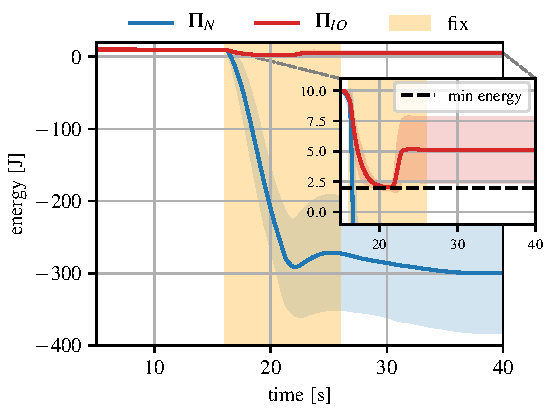
\includegraphics[width=0.8\linewidth]{figures/energy_with_without_tank.pdf}
    \caption{The energy of the tank when the filter is deployed (\textcolor{red}{\textbf{red}} curve) is always above the prescribed minimum, while it drastically drops in the other case. The plotted energy is computed integrating the dissipated power during interaction.}
\end{subfigure}
\hfill
\caption{The filter regulates the dissipated power when energy is low in the tank, resulting in a reduced wrench when the object is ``stuck". The line plot and shaded area show the mean and standard deviation from 20 simulation runs of interaction with the \textit{shelf} object respectively.}\label{fig:tank_comparison}
\end{figure}

\begin{figure}[t]
\centering
\includegraphics[width=0.8\columnwidth]{figures/passivity_coefficient_comparison.pdf}
\caption{In this figure we show the chattering effect happening when the constraints are enforced with $\alpha = 1/dt = 1000$. In contrast, a lower $\alpha$ greatly alleviates this issue.}\label{fig:tank_as_zbf}
\end{figure}

\vspace{0.3cm}
\subsubsection{Real-world experiments}
The goal of the hardware experiments is to demonstrate that the control framework can be deployed on a real platform in a real-time setup. For this purpose, we perform an interaction re-planning and a door opening experiment similar to the description provided in the previous section with our RoyalPanda robot. \addSecond{A video of the experiments can be found  \href{https://youtu.be/Q1AohXmsLs4}{here}}. The door displacement and the robot's base are tracked using a motion tracking system, eliminating the need for precise state estimation. We plan to remove this limitation in future work. 

\add{In the first hardware experiment, the} door motion is limited using a rope. \add{With this experiment we bring interaction to the limit case of extreme force applied to the articulation. Also, this situation might happen when a joint is stuck, e.g. because of stiction, wear and rust.} We monitor the evolution of the tank energy and once it has reached the allowed minimum we wait 3 seconds before manually cutting the rope. We repeat the experiment for the methods $\Pi_{N}$ and $\Pi_{IO}$ recalling that the latter only uses the passivity constraint in the inner loop.
%
The wrench norm and the evolution of the energy in the tank during the experiments can be seen in \fig \ref{fig:passivity_experiment}. As one can see in the accompanying video, without passivity, the manipulator exerts a rapidly increasing wrench until the rope is broken apart. On the other hand, when passivity is enforced, the power flow and external wrench is regulated leading to a robust interaction behavior and no need for the operator to intervene. When the object is released, the gripper gets stuck in a constrained configuration between the door plate and the handle. When $\Pi_{N}$ is deployed, the controller tries to push aggressively and is therefore not able to escape this gripper trap. Instead, when using $\Pi_{IO}$, the tank residual energy is low and aggressive actions are prohibited. The overall behavior is safer and allows the robot to escape from the bad configuration.  

\begin{figure}[t]
\centering
% \hspace*{-0.0cm} 
\begin{subfigure}{\columnwidth}
\centering
    \includegraphics[width=0.7\linewidth]{figures/wrench_norm.pdf}
    \caption{Wrench norm during the door opening experiment. We measure an average wrench of 68 N and 34 N for the $\Pi_{N}$ and $\Pi_{IO}$ methods respectively. The sharp wrench drop corresponds to the time when the rope breaks and energy is suddenly released. The two time series have been aligned to facilitate visualization.}
\end{subfigure}
% \hspace*{-0.2cm} 
\begin{subfigure}{\columnwidth}
\centering
    \includegraphics[width=0.7\linewidth]{figures/energy_tank.pdf}
    \caption{Evolution of the tank energy over time during the door opening experiment. The zoomed plot shows that energy is recovered when the object is released.}
\end{subfigure}
    \caption{The figures show that when passivity is enforced, the controller is able to limit the overall interaction wrench. This experiment is also reported in the accompanying video.}
    \label{fig:passivity_experiment}
\end{figure}


\add{In the second real-robot experiment, contained in the accompanying video, we aim to show the closed-loop and reactive nature of the control framework. During the experiment, the interaction with the articulated object is disturbed by a human operator, forcing the end effector to loose contact with the object handle. We observe that the controller is able to react and quickly find a new interaction strategy that achieves the task, while staying compliant at all times.}

% In order to qualitatively evaluate the algorithm's replanning capabilities, we disturb the manipulator during the opening phase, releasing the contact between the handle and the finger. As we can see in the accompanying video, the controller is able to re-plan a feasible trajectory to the handle and successfully perform the task. 

\section{Method Limitations and Future Work}\label{sec:limitations_and_future_works}
In the following we describe the most prominent issues that emerged during the experiments and how they could be addressed to improve the proposed method.

\subsection{Model Mismatch}
We have found that the method is highly sensitive to model mismatches. While we can assume that the robot model is known with high accuracy, this is often not the case for the object we intend to manipulate. Unfortunately, we observed that a small uncertainty in the estimate of the object pose and geometry could lead to failures in the door opening experiment. In particular, if the handle placement was not measured exactly, the controller would generate a ``tapping" motion which would cause a hard collision between the finger tip and the handle itself. One can try to quantify the sensitivity of the method to model mismatches and leverage this knowledge to account for the estimate uncertainty. Nevertheless this is not an easy task as there are dependencies across a range of factors, including the specific object geometry, finger design, object placement and articulation type. 

\subsection{State and Model Estimation}
We believe that a tighter integration with perception could be extremely fruitful and help to reduce the amount of prior knowledge needed. A perception system could be devised to extract local 3D patches that are used as candidate interaction hotspots. On the other hand, a surface mesh is not sufficient to model the object motion and dynamical behavior. As a matter of fact, an articulated object is also described by its kinematic parameters, namely the center and axis of rotation. Last but not least, mass, damping and friction could be estimated. However, since we did not tune any of these parameters to accurately match the real articulated object in our experiments, we conclude that the method is less sensitive to uncertainty in these model parameters.

\subsection{Cost Engineering}
The generation of good trajectories strongly depends on a well-engineered and task-dependent cost formulation. With poor cost tuning, stochastic policy optimization, as in the presented method, will tend to become trapped in local minima. Recall that during the manipulation task we rely mainly on two cost components. We use an end-effector pose cost to drive a virtual gripper frame to the location of an interaction frame, located on the medial axis of the handle. This serves as an interaction location prior. A second door-opening cost instead favors trajectories that pull the door open. If the first term is too high relative to the second, sampling could lead to sub-optimal solutions where the end-effector hovers in the proximity of the handle. In fact, pose deviations, from which some are able to successfully pull the door open, are highly penalized.

A second design aspect which influenced sampling quality is the placement of the virtual gripper frame. If this was too close to the finger collision geometry, random sampling would often fail to find a solution that avoids collision and successfully reaches the target pose. Instead, when this is placed at a small offset away from the finger tips one can prevent early collision and successfully reach the prescribed target pose. Both placements are shown in \fig \ref{fig:frame_placement}. While in this work we focus on a practical method for high-rate closed-loop control, a larger sampling budget or a multimodal policy distribution~\cite{lambert_stein_2020} could help to find better solutions but always at the cost of higher compute and lower control rates.

\begin{figure}[t]
\centering
\begin{subfigure}{0.48\columnwidth}
    \includegraphics[width=\linewidth]{figures/panda_grasp_2.png}
    \caption{Bad frame placement.}
\end{subfigure}%
\hfill
\begin{subfigure}{0.48\columnwidth}
    \includegraphics[width=\linewidth]{figures/panda_grasp_1.png}
    \caption{Good frame placement.}
\end{subfigure}%
\hfill
\caption{The location of the gripper frame used to compute the target reaching cost for manipulation can play a big role in finding a successful manipulation strategy.}\label{fig:frame_placement}
\end{figure}

In future work we would like to alleviate these issues by developing solutions that don't depend on more sampling and rather simplify cost engineering in a way to make it less sensitive to tuning and more generalizable across tasks. One way of achieving this goal would be to use a perception system to extract candidate interaction points and orientations from sensor data (as in~\cite{nagarajan2019grounded}), as an automated way of generating an ``interaction prior" in a continuous and real-time fashion. 

\subsection{Sim-to-real Gap}
Last but not least, particular care must be taken regarding the chosen physics engine used as a rollouts provider. Tuning is often required to reduce the compute time and allow for a longer prediction horizon. One simple way, also adopted in this work, is to increase the simulation step size at the cost of accuracy. This is in part compensated by the closed-loop nature of the control method that will reset the simulation to the newly observed robot state and therefore limit the simulation drift. Nowadays, there exists a plethora of physics engines that differ in algorithms, programming language and functionalities. A quantitative evaluation of the simulation accuracy and a comparative analysis is out of the scope of this work and recent reviews suggest that there isn't an obvious winner~\cite{collins2021review}. Nevertheless, when the task to solve is more complex, including contacts between more bodies and extends over a longer prediction horizon, we think that simulation fidelity can substantially improve the controller performance and therefore should be further investigated. 


\section{Conclusions} \label{sec:conclusions}
We have presented a novel control framework for interaction control. We have shown its applicability to the real platform and enhanced its robustness adding a safety layer which deploys ZBFs and passivity. Nevertheless there are still some interesting research directions that we aim to address in the near future. As any model-based control method, this is brittle to model mismatches. While stability is guaranteed through passivity, one could exploit interaction to find a better model estimate, closing the loop between perception and control. To this end, the haptic information readily available throughout the simulated rollouts could be actively used to drive an exploratory behavior. Another interesting idea is the use of a different policy parametrization than a multivariate gaussian such that sampling could be done more efficiently in a lower dimensional space. The proposed method is flexible enough to be applied to other system than mobile manipulators. We hope that the released library will help in this process and development of future applications. 


% \addtolength{\textheight}{-13.5cm}   % This command serves to balance the column lengths
                                  % on the last page of the document manually. It shortens
                                  % the textheight of the last page by a suitable amount.
                                  % This command does not take effect until the next page
                                  % so it should come on the page before the last. Make
                                  % sure that you do not shorten the textheight too much.

%%%%%%%%%%%%%%%%%%%%%%%%%%%%%%%%%%%%%%%%%%%%%%%%%%%%%%%%%%%%%%%%%%%%%%%%%%%%%%%%
% \section*{ACKNOWLEDGMENT}

% This work was supported in part by ABB Corporate Research, the Luxembourg National Research Fund (FNR) 12571953 and the ETH Foundation with an unrestricted gift from Huawei Technologies.


%%%%%%%%%%%%%%%%%%%%%%%%%%%%%%%%%%%%%%%%%%%%%%%%%%%%%%%%%%%%%%%%%%%%%%%%%%%%%%%%

\bibliographystyle{IEEEtran}
% argument is your BibTeX string definitions and bibliography database(s)
\bibliography{references}

%%%%%%%%%%%%%%%%%%%%%%%%%%%%%%%%%%%%%%%%%%%%%%%%%%%%%%%%%%%%%%%%%%%%%%%%%%%%%%%%
\appendices
\section{Derivation of policy gradient}\label{sec:app_derivation_policy_gradient}
Recall that the optimization variables are the parameters of the current policy, namely the mean vector of the normally distributed control sequence $\policyParams = \bar{\boldsymbol{\mu}} = \{\boldsymbol{\mu}_t,  \boldsymbol{\mu}_{t+1}, \dots, \boldsymbol{\mu}_{t+T-1} \}$. For a input command at time $k$ in the horizon, $\command_k \sim \mathcal{N}(\boldsymbol{\mu}_k, \Sigma)$. Recall also that we map costs to \emph{success likelihoods} using the exponential function $\succCondProb = \exp(-\lambda J(X_t, U_t)) = \mathcal{J}_t$ . We show the derivation of the gradient for one nominal input vector $\boldsymbol{\mu}_k$:

\begin{align}
    \nabla_{\boldsymbol{\mu}_k} \log \expPolicy{\succCondProb}
    &= \frac{\nabla_{\boldsymbol{\mu}_k} \expPolicy{\succCondProb}}{\expPolicy{\succCondProb}} \\
    &= \frac{\nabla_{\boldsymbol{\mu}_k} \expPolicy{\mathcal{J}_t}}{\expPolicy{\mathcal{J}_t}} \label{eq:log_gradient}
\end{align}

 We further expand the numerator in the previous expression:
\begin{align}
    \nabla_{\boldsymbol{\mu}_k} \expPolicy{\mathcal{J}_t} 
    &= \nabla_{\boldsymbol{\mu}_k} \int \mathcal{J}_t \policy(U_t) \label{eq:param_independence}\\
    &= \int \mathcal{J}_t \nabla_{\boldsymbol{\mu}_t} \policy(U_t) \\
    &= \int \mathcal{J}_t \policy(U_t) \nabla_{\boldsymbol{\mu}_k} \log \policy(U_t) \\
    &= \expectation{\policy} [\mathcal{J}_t \nabla_{\boldsymbol{\mu}_k} \log \policy(U_t)] \label{eq:almost_there}
\end{align}
where the step \eqref{eq:param_independence} follows from the independence of the success likelihood from the policy parameters. We now look at the gradient of the policy log-likelihood with respect to the mean vector:
\begin{align}
    &\nabla_{\boldsymbol{\mu}_k} \log \policy(U_t) \\
    &= \nabla_{\boldsymbol{\mu}_k} \log \prod_{t}^{T+t-1} \frac{1}{\sqrt{(2\pi)^{n_u}|\variance|}}\exp\left(-\frac{1}{2}||\command_t - \boldsymbol{\mu}_t||_{\variance^{-1}}\right) \\
    &= \nabla_{\boldsymbol{\mu}_k} \sum_{t}^{T+t-1} \log \frac{1}{\sqrt{(2\pi)^{n_u}|\variance|}} + \left(-\frac{1}{2}||\command_t - \boldsymbol{\mu}_t||_{\variance^{-1}}\right) \\
    &= \nabla_{\boldsymbol{\mu}_k} \sum_{t}^{T+t-1} -\frac{1}{2}||\command_t - \boldsymbol{\mu}_t||_{\variance^{-1}} \\
    &= \nabla_{\boldsymbol{\mu}_k} -\frac{1}{2}||\command_k - \boldsymbol{\mu}_k||_{\variance^{-1}} \\
    &= \variance^{-1}(\command_k - \boldsymbol{\mu}_k) \\
    &= \variance^{-1} \noise_k
\end{align}
Plugging the previous expression in \eqref{eq:almost_there} we obtain:
\begin{align}
    \expectation{\boldsymbol{\mu}_k} [\mathcal{J}_t \nabla_{\boldsymbol{\mu}_k} \log \policy(U_t)]
    &= \expectation{\policy} [\mathcal{J}_t \variance^{-1} \noise_k] \\
    &= \variance^{-1} \expPolicy{\mathcal{J}_t \noise_k} \label{eq:mean_gradient}
\end{align}
We finally combine \eqref{eq:mean_gradient} and \eqref{eq:log_gradient} to get the equation which relates the gradient to the cost and input noise:
\begin{align}
     \nabla_{\boldsymbol{\mu}_k} \log \expPolicy{\succCondProb} 
     &= \variance^{-1} \frac{\expPolicy{\mathcal{J}_t \noise_k}}{\expPolicy{\mathcal{J}_t}} \\
     &= \variance^{-1} \frac{\expPolicy{\exp(-\lambda J_t) \noise_k}}{\expPolicy{\exp(-\lambda J_t)}}
\end{align}


\section{Table of parameters}\label{app:table_of_parameters}

\begin{table}[h!]
\centering
\begin{tabular}{c c c c}
 \toprule
 Col1 & Col2 & Col2 & Col3 \\ [0.5ex] 
 \midrule
 1 & 6 & 87837 & 787 \\ 
 
 2 & 7 & 78 & 5415 \\
 
 3 & 545 & 778 & 7507 \\
 
 4 & 545 & 18744 & 7560 \\
 
 5 & 88 & 788 & 6344 \\ [1ex] 
 \bottomrule
\end{tabular}
\caption{Table to test captions and labels.} \label{ta}
\label{tab:parameters}
\end{table}


%%%%%%%%%%%%%%%%%%%%%%%%%%%%%%%%%%%%%%%%%%%%%%%%%%%%%%%%%%%%%%%%%%%%%%%%%%%%%%%%

% References are important to the reader; therefore, each citation must be complete and correct. If at all possible, references should be commonly available publications.
\vspace{-1cm}
\begin{IEEEbiography}[{\includegraphics[width=1in,height=1.25in,clip,keepaspectratio]{figures/biographies/grizzi.jpg}}]{Giuseppe Rizzi}
is a PhD student in the Autonomous System Lab at ETH Zürich. He received a B.Sc in Mechanical Engineering at Politecnico di Milano in 2016 and a M.Sc in Robotics, Systems and Control at ETH Zürich in 2019. He joined the Robotic Systems Lab (RSL) as a Research Assistant and worked on autonomous navigation and manipulation for the MBZIRC competition in 2019. In 2020 he started is PhD program and joined the Mobile Manipulation Team. His research interests include control and perception for robotic manipulation.  
\end{IEEEbiography}

\begin{IEEEbiography}[{\includegraphics[width=1in,height=1.25in,clip,keepaspectratio]{figures/biographies/jjchung.jpg}}]{Jen Jen Chung}
(Member, IEEE) is an Associate Professor in Mechatronics within the School of Information Technology and Electrical Engineering at The University of Queensland. Her current research interests include perception, planning and learning for robotic mobile manipulation, algorithms for robot navigation through human crowds, informative path planning and adaptive sampling. Prior to working at UQ, Jen Jen was a Senior Researcher in the Autonomous Systems Lab (ASL) at ETH Zürich from 2018-2022 and was a postdoctoral scholar at Oregon State University researching multiagent learning methods from 2014-2017. She completed her Ph.D. on information-based exploration-exploitation strategies for autonomous soaring platforms at the Australian Centre for Field Robotics in the University of Sydney. She received her Ph.D. (2014) and B.E. (2010) from the University of Sydney.
\end{IEEEbiography}
\vspace{-1cm}
\begin{IEEEbiography}[{\includegraphics[width=1in,height=1.25in,clip,keepaspectratio]{figures/biographies/gawela.jpg}}]{Abel Gawel} is currently a Principal Researcher in Computer Vision and Machine Learning with the Huawei European Research Center. Before that he was a Senior Scientist at the Autonomous Systems Lab of ETH Zurich. He received the PhD from ETH Zurich in 2018 and was a visiting Postdoctoral Fellow in the CRI group at NTU Singapore in 2019. His research interests include SLAM, high-accuracy localization, object recognition, and semantic scene understanding with application in construction robotics, industrial inspection, and search and rescue robotics. Prior to joining ETH in 2014, he worked for Bosch Corporate Research and the BMW group.
\end{IEEEbiography}
\vspace{-1cm}
\begin{IEEEbiography}[{\includegraphics[width=1in,height=1.25in,clip,keepaspectratio]{figures/biographies/2020_Marco_Tognon_3.jpg}}]{Marco Tognon}
(S'15-M'18) from November 2022 is a tenuered researcher at INRIA Rennes, France, in the Rainbow team. Before he was a postdoctoral researcher in the Autonomous System Lab (ASL) at ETH Zurich, Switzerland.
He received the Ph.D.~degree in Robotics in 2018, from INSA Toulouse, France, developing his thesis at LAAS-CNRS.
His thesis has been awarded with three prizes. 
He received the M.Sc. degree in automation engineering in 2014, from the University of Padua, Italy, with a master thesis carried out at MPI for Biological Cybernetics, T\"ubingen, Germany.
From 2018 to 2020 he has been postdoctoral researcher at LAAS-CNRS, Toulouse, France. 
%Since 2020 he is postdoctoral researcher at ETH Zurich, Switzerland, in the ASL group.
His current research interests include robotics, aerial physical interaction, multi-robot systems, and human-robot physical interaction.
\end{IEEEbiography}
\vspace{-1cm}
\begin{IEEEbiography}[{\includegraphics[width=1in,height=1.25in,clip,keepaspectratio]{figures/biographies/lott.jpg}}]{Lionel Ott} is a Senior Researcher in the Autonomous Systems Lab (ASL) at ETH Zurich. His research focuses on the intersection between machine learning and robotics with the goal to develop methods, techniques, and systems that allow an autonomous agent to build and maintain a representation of the ever-changing world in which robotics systems operate to achieve their given task. His interests are in model learning and decision making, taking uncertainty into account. Before working at ASL, Lionel was a senior research fellow in the School of Computer Science at the University of Sydney. He received his Ph.D. in 2014 from the University of Sydney.
\end{IEEEbiography}
\vspace{-1cm}
\begin{IEEEbiography}[{\includegraphics[width=1in,height=1.25in,clip,keepaspectratio]{figures/biographies/rsiegwart.jpg}}]{Roland Siegwart}
(Fellow, IEEE) is a Professor for autonomous mobile robots with ETH Zurich, Founding Co-Director of the Technology Transfer Center, Wyss Zurich and Board Member of multiple high-tech companies. From 1996 to 2006, he was a Professor with EPFL Lausanne, held visiting positions with Stanford University and NASA Ames and was Vice President of ETH Zurich from 2010 to 2014. His research interest include the design, control, and navigation of flying, and wheeled and walking robots operating in complex and highly dynamical environments.

Prof. Siegwart received the IEEE RAS Pioneer Award and IEEE RAS Inaba Technical Award. He is among the most cited scientist in robots world-wide, Co-Founder of more than half a dozen spin-off companies, and a strong promoter of innovation and entrepreneurship in Switzerland.
\end{IEEEbiography}
\vfill
\end{document}
